% !TEX root = ../OT4ML.tex

%%%%%%%%%%%%%%%%%%%%%%%%%%%%%%%%%%%%%%%%%%%%%%%%%%%%%%%%%%%%%%%%%%%%%%%%%%%
%%%%%%%%%%%%%%%%%%%%%%%%%%%%%%%%%%%%%%%%%%%%%%%%%%%%%%%%%%%%%%%%%%%%%%%%%%%
%%%%%%%%%%%%%%%%%%%%%%%%%%%%%%%%%%%%%%%%%%%%%%%%%%%%%%%%%%%%%%%%%%%%%%%%%%%
\chapter{Entropic Regularization: Convergence}
\index{entropic!regularization}% strictindex
\index{Sinkhorn!convergence}% strictindex
\label{sec-sinkhorn-advanced}
\label{sec-entropic-convergence}
\label{sec-convergence-dual}

This chapter focuses on algorithmic convergence for entropic optimal transport: the marginals and the temperature are fixed, and one asks how Sinkhorn iterates, soft transforms and related monotone scaling procedures approach their regularized fixed point. Statistical convergence is a separate question, because the empirical marginals then change with the sample size; this is the topic of Chapter~\ref{sec-statistical-ot}.
\index{algorithmic convergence}% strictindex
\index{Sinkhorn!fixed point}% strictindex
\index{matrix!scaling}% strictindex
\index{soft!transform}% strictindex

The chapter revisits Sinkhorn convergence through several complementary lenses. Bregman projections explain the alternating-projection geometry, Fortet's order argument gives qualitative fixed-point convergence, and an order-theoretic M-function viewpoint explains why Sinkhorn-like scaling can still converge even when the equations are no longer the gradient of a convex potential. Robust Bregman estimates then give a non-asymptotic $O(1/k)$ dual-gap bound, while Hilbert's metric gives a clean linear contraction when the kernel is uniformly positive. The last sections discuss Gaussian closed forms and continuous \(\varepsilon\)-Sinkhorn flows as model cases where the fixed-point structure becomes explicit.
\index{Sinkhorn!convergence}% strictindex
\index{Bregman!projection}% strictindex
\index{dual!gap}% strictindex
\index{M-function}% strictindex

%%%%%%%%%%%%%%%%%%%%%%%%%%%%%%%%%%%%%%%%%%%%%%%%%%%%%%%%%%%%%%%%%%%%%%%%%%%
\section{Sinkhorn Convergence: Bregman Point of View}
\label{sec-convergence-init}

This section explains Sinkhorn as alternating Bregman projections. The main message is geometric: each row or column rescaling is the KL projection onto one affine marginal constraint, so convergence follows from the Pythagorean identity for Bregman divergences.
\index{KL!projection}% strictindex
\index{marginal!constraint}% strictindex
\index{affine!marginal constraint}% strictindex
\index{Pythagorean identity}% strictindex
\index{Bregman!divergence}% strictindex
\index{Bregman!projection}% strictindex

For simplicity, this section is written for discrete measures, but the same ideas carry over to general measures. The robust-rate section later revisits the alternating-projection mechanism through convex duality, with constants expressed through the oscillation of the potentials and of the cost range.

%%%%
\paragraph{Alternating $\KL$ projections.}
\index{alternating!projection}% strictindex

The projection viewpoint explains Sinkhorn as repeated enforcement of one marginal constraint at a time. It is not specific to entropy, although the KL case is the one where the projections reduce to elementary row and column scalings.
\index{scaling!row}% strictindex
\index{scaling!column}% strictindex
\index{marginal!constraint}% strictindex

\begin{defn}[Bregman divergence]\label{def-bregman-divergence}
\index{Bregman!divergence}% strictindex
	Let $\Phi$ be a differentiable strictly convex function on the interior of a convex domain $\Omega$. For $\P,Q\in\operatorname{int}(\Omega)$, the Bregman divergence generated by $\Phi$ is
\index{convex!function}% strictindex
	\[
		B_\Phi(\P|Q)\eqdef \Phi(\P)-\Phi(Q)-\dotp{\nabla\Phi(Q)}{\P-Q}.
	\]
	For the negative entropy $\Phi(\P)=\sum_{i,j}\P_{i,j}\log \P_{i,j}$ on the positive orthant, this gives $B_\Phi(\P|Q)=\KLD(\P|Q)$. The same formula extends lower-semicontinuously to $\P\geq0$ when $Q>0$, with $0\log0=0$.
\index{negative Shannon entropy}% strictindex
\end{defn}

The corresponding projection is the basic operation in alternating Bregman methods.
\begin{defn}[Bregman projection]\label{def-bregman-projection}
For a nonempty convex set $\Cc$, define
\[
	\Proj_{\Cc}^{B_\Phi}(\Q)
	\eqdef
	\argmin_{\P\in\Cc} B_\Phi(\P|\Q),
\]
which is set-valued if the minimizer is not unique.
\end{defn}

Bregman divergences are useful because their geometry can encode constraints. A Legendre-type generator $\Phi$ blows up, or has an infinite derivative, at the boundary of its domain. For negative entropy, positivity is therefore built into the divergence, so one projects onto affine marginal constraints without separately handling non-negativity.
\index{affine!marginal constraint}% strictindex
\index{marginal!constraint}% strictindex
\index{Bregman!divergence}% strictindex

\paragraph{Linear tilts and Gibbs references.}
\index{linear!tilt}% strictindex
\index{Gibbs!reference}% strictindex

The next proposition explains why adding a linear cost to a Bregman penalty merely shifts the reference point in dual coordinates. The usual Gibbs--KL reformulation is the entropy specialization.

\begin{prop}[Linear tilts of Bregman penalties]\label{prop-bregman-linear-tilt}
\index{Bregman!penalty}% strictindex
	Let $\Phi$ be differentiable and strictly convex, and let $B_\Phi$ be its Bregman divergence. Fix a reference point $\Q$ in the interior of the domain. Assume that there exists $\Q^\C$ such that
\index{Bregman!divergence}% strictindex
	\[
		\nabla\Phi(\Q^\C)=\nabla\Phi(\Q)-\C/\epsilon .
	\]
	Then, for all $\P$ in the domain,
	\[
		\dotp{\P}{\C}+\epsilon B_\Phi(\P|\Q)
		=
		\epsilon B_\Phi(\P|\Q^\C)+\text{\upshape cst},
	\]
	where the constant does not depend on $\P$.
\end{prop}
\begin{proof}
	Subtract the two Bregman divergences:
\index{Bregman!divergence}% strictindex
	\[
		B_\Phi(\P|\Q^\C)-B_\Phi(\P|\Q)
		=
		\dotp{\nabla\Phi(\Q)-\nabla\Phi(\Q^\C)}{\P}
		+\text{cst}.
	\]
	Using $\nabla\Phi(\Q)-\nabla\Phi(\Q^\C)=\C/\epsilon$ and multiplying by $\epsilon$ gives the claim.
\end{proof}

For the negative entropy $\Phi(\P)=\sum_{i,j}\P_{i,j}\log\P_{i,j}$, one has $B_\Phi=\KLD$. Taking $\Q=\a\otimes\b$ gives the tilted reference
\index{negative Shannon entropy}% strictindex
\[
	\K_{\a,\b}^\epsilon
	\eqdef
	(\a\otimes\b)\odot e^{-\C/\epsilon}.
\]
Thus
\[
	\dotp{\P}{\C}+\epsilon\KLD(\P|\a\otimes\b)
	=
	\epsilon\KLD(\P|\K_{\a,\b}^\epsilon)+\text{\upshape cst}.
\]
On the transport polytope, scaling $\K_{\a,\b}^\epsilon$ is equivalent to scaling the Gibbs kernel $\K=e^{-\C/\epsilon}$ because the factors $\a_i$ and $\b_j$ can be absorbed into the Sinkhorn scalings.
\index{Sinkhorn!scaling}% strictindex
\index{transportation polytope}% strictindex
\index{Gibbs!kernel}% strictindex

Thus the unique solution $\P_\epsilon$ of~\eqref{eq-regularized-discr} is the KL projection of the tilted Gibbs reference onto $\CouplingsD(\a,\b)$:
\index{Gibbs!reference}% strictindex
\index{KL!projection}% strictindex
\eql{\label{eq-kl-proj}
	\P_\epsilon = \Proj_{\CouplingsD(\a,\b)}^\KLD(\K_{\a,\b}^\epsilon) \eqdef \uargmin{\P \in \CouplingsD(\a,\b)} \KLD(\P|\K_{\a,\b}^\epsilon).
}

\paragraph{Cyclic projection convergence.}
\index{cyclic!projection}% strictindex

The convergence mechanism is the classical one of Bregman~\cite{bregman1967relaxation}.

\begin{prop}[Cyclic Bregman projections on affine constraints]\label{prop-cyclic-kl-affine}
\index{Bregman!projection}% strictindex
\index{affine!constraint}% strictindex
	Let $\Phi$ be a Legendre strictly convex generator on a finite-dimensional convex domain, and let $\Cc_1,\Cc_2$ be affine constraint sets whose intersection meets the interior of the domain. Define
	\[
		\P^{(\ell+1)}
		=
		\Proj_{\Cc_2}^{B_\Phi}
		\Proj_{\Cc_1}^{B_\Phi}(\P^{(\ell)}),
	\]
	starting from an interior point $\P^{(0)}$. Assume that the projections are well-defined and that the half-step sequence remains in a compact subset of the interior of the domain. Then $\P^{(\ell)}$ converges to the Bregman projection of $\P^{(0)}$ onto $\Cc_1\cap\Cc_2$.
\index{affine!marginal constraint}% strictindex
\index{transportation polytope}% strictindex
\index{marginal!constraint}% strictindex
\index{Bregman!projection}% strictindex
\end{prop}
\begin{proof}
	We first prove the Pythagorean identity used by the projection argument. For three interior points one has the Bregman three-point formula
\index{Bregman!three-point formula}% strictindex
\index{Pythagorean identity}% strictindex
	\[
		B_\Phi(Q|\P)
		=
		B_\Phi(Q|\P^+)
		+
		B_\Phi(\P^+|\P)
		+
		\dotp{\nabla\Phi(\P^+)-\nabla\Phi(\P)}{Q-\P^+}.
	\]
	If $\P^+=\Proj_\Cc^{B_\Phi}(\P)$ and $\Cc$ is affine, the first-order optimality condition for minimizing $R\mapsto B_\Phi(R|\P)$ over $R\in\Cc$ is
\index{optimality!first-order}% strictindex
	\[
		\dotp{\nabla\Phi(\P^+)-\nabla\Phi(\P)}{R-\P^+}=0
		\qquad \forall R\in\Cc,
	\]
	because $R-\P^+$ ranges over the tangent linear space of $\Cc$. Taking $R=Q\in\Cc$ cancels the last term and gives
	\[
		B_\Phi(Q|\P)=B_\Phi(Q|\P^+)+B_\Phi(\P^+|\P)
		\qquad\forall Q\in\Cc.
	\]

	Let $(Z^{(r)})_r$ be the half-step sequence obtained by alternating projections onto $\Cc_1$ and $\Cc_2$, so that $Z^{(2\ell)}=\P^{(\ell)}$ and $Z^{(2\ell+2)}=\P^{(\ell+1)}$. Fix $Q\in\Cc_1\cap\Cc_2$. Applying the identity at each half-step gives
\index{Sinkhorn!half-step}% strictindex
\index{alternating!projection}% strictindex
	\[
		B_\Phi(Q|Z^{(r)})-B_\Phi(Q|Z^{(r+1)})
		=
		B_\Phi(Z^{(r+1)}|Z^{(r)})\geq0.
	\]
	Thus $B_\Phi(Q|Z^{(r)})$ decreases and the series $\sum_r B_\Phi(Z^{(r+1)}|Z^{(r)})$ is finite. The compactness assumption gives cluster points. Since the projection drops tend to zero and $\Phi$ is strictly convex on compact subsets of the domain, $\norm{Z^{(r+1)}-Z^{(r)}}\to0$. Every cluster point of the even subsequence is therefore also a cluster point of the adjacent odd subsequence. Because these two subsequences lie alternately in the closed affine sets $\Cc_1$ and $\Cc_2$, every cluster point belongs to $\Cc_1\cap\Cc_2$.

	Let $\bar \P$ be such a cluster point. For each half-step, the dual displacement
\index{Sinkhorn!half-step}% strictindex
	\(\nabla\Phi(Z^{(r+1)})-\nabla\Phi(Z^{(r)})\)
	belongs to the normal space of the affine set onto which one projects. Telescoping and using the convergence of $Z^{(r)}$ gives
	\[
		\nabla\Phi(\bar \P)-\nabla\Phi(\P^{(0)})
		\in
		N_{\Cc_1}+N_{\Cc_2}
		=
		N_{\Cc_1\cap\Cc_2},
	\]
	where the last equality uses that the sets are affine. This is precisely the first-order optimality condition for minimizing $R\mapsto B_\Phi(R|\P^{(0)})$ over $R\in\Cc_1\cap\Cc_2$. Thus $\bar \P$ is the Bregman projection of $\P^{(0)}$ onto the intersection. Strict convexity gives uniqueness of this minimizer, so all cluster points coincide and the whole sequence converges.
\index{negative Shannon entropy}% strictindex
\index{optimality!first-order}% strictindex
\index{Bregman!projection}% strictindex
\index{strict!convexity}% strictindex
\end{proof}

\begin{alg}[Cyclic Bregman projections]\label{alg:cyclic-bregman-projections}
\index{cyclic!Bregman projection}% strictindex
\textbf{Input:} Constraint sets $\Cc_1,\Cc_2$, Bregman divergence $B_\Phi$, interior point $\P^{(0)}$, constraint defects \(\mathrm{def}_{\Cc_1},\mathrm{def}_{\Cc_2}\), tolerance $\mathrm{tol}$, iteration budget $L\geq1$.

\textbf{Output:} Point in $\Cc_1\cap\Cc_2$ when the intersection is feasible.

\textbf{Specialize} to entropic OT, if needed:
\(\Cc_1=\Cc^1_\a, \qquad \Cc_2=\Cc^2_\b, \qquad B_\Phi=\KL.\)

\textbf{Initialize:} Set \(r^{(0)}=+\infty\) and \(\ell=0\).

\textbf{While} \(r^{(\ell)}>\mathrm{tol}\) and $\ell<L$ \textbf{do}:
\begin{algblock}

\textbf{Set} \(\ell\leftarrow \ell+1\).

\(\P^{(\ell-1/2)}=\Proj_{\Cc_1}^{B_\Phi}(\P^{(\ell-1)}).\)

\(\P^{(\ell)}=\Proj_{\Cc_2}^{B_\Phi}(\P^{(\ell-1/2)}).\)

\textbf{Set} \(r^{(\ell)}=\max\{\mathrm{def}_{\Cc_1}(\P^{(\ell)}),\mathrm{def}_{\Cc_2}(\P^{(\ell)})\}\).
\end{algblock}
\algreturnskip
\textbf{Return} $\P^{(\ell)}$.
\end{alg}

Denoting
\eq{
	\Cc^1_\a \eqdef \enscond{\P}{\P\ones_m=\a}
	\qandq
	\Cc^2_\b \eqdef \enscond{\P}{\transp{\P}\ones_n=\b}
}
the rows and columns constraints, one has $\CouplingsD(\a,\b) = \Cc^1_\a \cap \Cc^2_\b$. One can use KL, or more generally Bregman, iterative projections~\cite{bregman1967relaxation,Ruschendorf95,RuschendorfThomsen}
\eql{\label{eq-kl-sinkh-proj}
	\itt{\P} \eqdef \Proj_{\Cc^1_\a}^{\KLD}(\it{\P})
	\qandq
	\ittt{\P} \eqdef \Proj_{\Cc^2_\b}^{\KLD}(\itt{\P}).
}
For positive histograms and a strictly positive Gibbs kernel, the classical iterative-proportional-fitting theorem ensures that the KL half-steps remain in the positive stratum and converge~\cite{Ruschendorf95,RuschendorfThomsen}. Proposition~\ref{prop-cyclic-kl-affine}, applied with $\P_0=\K_{\a,\b}^\epsilon$, then identifies the limit as the KL projection~\eqref{eq-kl-proj}. The Hilbert-metric argument in Section~\ref{sec-sinkhorn-hilbert} gives an independent quantitative proof.

\paragraph{Row and column scalings.}
\index{scaling!row}% strictindex
\index{scaling!column}% strictindex

The two projectors are simple to compute since they correspond to scaling respectively the rows and the columns, as explained in this proposition.

\begin{prop}[KL projections are scalings]
\index{KL!projection}% strictindex
One has
\eq{
	 \Proj_{\Cc^1_\a}^{\KLD}(\P) = \diag\pa{\frac{\a}{\P \ones_m}} \P
	 \qandq
	 \Proj_{\Cc^2_\b}^{\KLD}(\P) =  \P \diag\pa{\frac{\b}{\P^\top \ones_n}}.
}
\end{prop}
\begin{proof}
	Consider the problem along each row or column vector to impose a fixed sum $s \in \RR_+$
	\(\umin{p} \enscond{\KL(p|q)}{\dotp{p}{\ones}=s}\).
	The Lagrange multiplier equation for this problem reads
	\eq{
		\log(p/q)+\la \ones=0 \qarrq
		p = u q \qwhereq u = e^{-\la}>0.
	}
	The constraint $\dotp{p}{\ones} = s$ is equivalent to $\dotp{uq}{\ones}=s$, i.e. $u=s/\sum_i q_i$, which gives the desired scaling formula
\index{scaling!form}% strictindex
	$p=s q/\sum_i q_i$.
\end{proof}

These iterations are equivalent to Sinkhorn iterations~\eqref{eq-sinkhorn} since defining
\index{Sinkhorn!iteration}% strictindex
\eq{\label{eq-sink-matrix}\P^{(2\ell)} \eqdef \diag(\it{\uD}) \K \diag(\it{\vD}),}
one has
\begin{align*}
	\P^{(2\ell+1)} &\eqdef \diag(\itt{\uD}) \K \diag(\it{\vD}) \\
	\qandq
	\P^{(2\ell+2)} &\eqdef \diag(\itt{\uD}) \K \diag(\itt{\vD})
\end{align*}
In practice, however, one should prefer using~\eqref{eq-sinkhorn}, which only requires manipulating scaling vectors and multiplying by a Gibbs kernel, and can often be accelerated when the kernel has separable, sparse, low-rank or geometric structure.
\index{scaling!vectors}% strictindex
\index{Gibbs!kernel}% strictindex

Such a convergence analysis using Bregman projection is of limited interest because it only works directly in finite dimension. For instance, the linear convergence speed one can obtain from strong convexity degrades with the dimension and with $\epsilon$. The robust dual analysis below gives a dimension-free qualitative message: the constants are expressed through the oscillation of the potentials and the cost range, and the resulting $O(1/k)$ estimate explains what can be guaranteed before any asymptotic linear regime becomes visible.
\index{Bregman!projection}% strictindex
\index{linear!convergence}% strictindex
%
It is also possible to anneal $\epsilon$ during the iterations and to rely on multiscale strategies in low dimensions.

%%%%%%%%%%%%%%%%%%%%%%%%%%%%%%%%%%%%%%%%%%%%%%%%%%%%%%%%%%%%%%%%%%%%%%%%%%%
\section{Sinkhorn Convergence: Monotone Point of View}\label{sec-sinkhorn-monotone}
\index{monotone!convergence}% strictindex
\index{Sinkhorn!convergence}% strictindex

This section isolates the order structure of Sinkhorn's potential updates. The one-sided soft transforms reverse order, whereas a full cycle preserves order and commutes with additive constants. This yields a monotone convergence route from subsolutions and, more generally, a gauge-invariant nonexpansiveness principle.

\paragraph{Fortet monotonicity.}
\index{Fortet iteration}% strictindex
There is another, older way to understand convergence, going back to Fortet's proof of the Schr\"odinger system~\cite{fortet1940schrodinger,essid2019fortet,leonard2019fortet}. It does not primarily estimate a contraction factor. Instead, it uses the order structure of the soft transforms.
\index{Schrodinger@Schr\"odinger!system}% strictindex
\index{soft!transform}% strictindex

\begin{prop}[Monotone fixed-point route to Sinkhorn convergence]\label{prop-fortet-monotone}
\index{monotone!fixed point}% strictindex
	Let $c$ be bounded and continuous on compact spaces, and define the unnormalized double Sinkhorn map
	\[
		\mathcal A(f) \eqdef (f^{c,\epsilon})^{\bar c,\epsilon}.
	\]
	The map $\mathcal A$ is order preserving and additively homogeneous:
	\[
		f\leq h\Longrightarrow \mathcal A(f)\leq\mathcal A(h),
		\qquad
		\mathcal A(f+\lambda)=\mathcal A(f)+\lambda.
	\]
	Let $f^\star$ be an entropic fixed point and suppose that $f^{(0)}$ is a subsolution, meaning $f^{(0)}\leq\mathcal A(f^{(0)})$. After subtracting a sufficiently large constant from $f^{(0)}$, which preserves the subsolution inequality, assume $f^{(0)}\leq f^\star$. Then the iterates $f^{(\ell+1)}=\mathcal A(f^{(\ell)})$ increase pointwise, remain bounded above by $f^\star$, and converge uniformly to an entropic fixed point. Their classes modulo constants therefore converge to the unique entropic potential class.
\index{Sinkhorn!scaling}% strictindex
\index{order-preserving map}% strictindex
\index{entropic!potential}% strictindex
\end{prop}

\begin{proof}
	The soft $c$-transform is order reversing: if $g\leq g'$, then
\index{soft!c-transform}% strictindex
	\[
		-\epsilon\log\int e^{(g-c)/\epsilon}\d\be
		\geq
		-\epsilon\log\int e^{(g'-c)/\epsilon}\d\be.
	\]
	The composition of two order-reversing transforms is order preserving. Since each one-sided transform is additively anti-homogeneous, their composition is additively homogeneous. The subsolution inequality gives $f^{(0)}\leq f^{(1)}$; order preservation then yields $f^{(\ell)}\leq f^{(\ell+1)}$ for every $\ell$. Likewise, $f^{(0)}\leq f^\star$ implies $f^{(\ell)}\leq\mathcal A^\ell(f^\star)=f^\star$. Thus $(f^{(\ell)})_\ell$ converges pointwise. All $f^{(\ell)}$ with $\ell\geq1$ are double soft transforms, so their oscillations and moduli of continuity are controlled by those of the bounded continuous cost. Arzel\`a--Ascoli makes the convergence uniform, and continuity of $\mathcal A$ shows that the limit is a fixed point. Proposition~\ref{prop-entropic-dual-potentials} identifies all continuous fixed points up to constants, while Proposition~\ref{prop-entropic-unique} identifies their common coupling.
\index{order-preserving map}% strictindex
\index{entropic!potential}% strictindex
\index{soft!transform}% strictindex
\end{proof}

The subsolution condition is invariant under additive shifts: shifting a function can place it below a fixed point, but cannot turn a non-subsolution into a subsolution. Convergence from an arbitrary initialization follows from the compactness-and-dual-ascent argument in Fortet's theorem, or from the Hilbert contraction below, rather than from this monotone sandwich alone~\cite{fortet1940schrodinger,essid2019fortet,leonard2019fortet}. The proposition isolates the genuinely order-theoretic part of that mechanism.
\index{alternating!projection}% strictindex

\paragraph{Extension beyond KL.}
\index{phi-divergence regularized OT}% strictindex
\index{soft!c-transform}% strictindex
The monotone argument is not specific to the exponential law of KL regularization. For the $\phi$-divergence regularized problems of Section~\ref{sec-sinkhorn-other-regularizers}, write
\[
	\Phi_\phi\eqdef \phi^*.
\]
The Fenchel dual ascent updates are the generalized soft $c$-transforms. For fixed $g$, the update of $f$ is the function
\[
	g^{\bar c,\epsilon,\phi}(x)
	\in
	\uargmin{u\in\RR}
	\left\{
		\epsilon
		\int_{\Yy}
		\Phi_\phi\!\left(\frac{u+g(y)-c(x,y)}{\epsilon}\right)
		\d\be(y)
		-u
	\right\},
\]
which is the same formula as~\eqref{eq-phi-soft-c-transform}. The update $f^{c,\epsilon,\phi}$ is obtained by exchanging $(x,\al,f)$ and $(y,\be,g)$. In nonsmooth cases the scalar optimality condition is the subgradient normalization
\[
	1\in
	\int_{\Yy}
		\partial\Phi_\phi\!\left(\frac{g^{\bar c,\epsilon,\phi}(x)+g(y)-c(x,y)}{\epsilon}\right)
	\d\be(y),
	\qquad
	1\in
	\int_{\Xx}
		\partial\Phi_\phi\!\left(\frac{f(x)+f^{c,\epsilon,\phi}(y)-c(x,y)}{\epsilon}\right)
	\d\al(x),
\]
where the integral of intervals is understood in the usual Aumann sense, under the standard qualification allowing subdifferentiation under the integral. When $\Phi_\phi$ is differentiable and $\rho_\phi\eqdef\Phi_\phi'$, this becomes the normalization relations
\[
	\int_{\Yy}
	\rho_\phi\!\left(\frac{g^{\bar c,\epsilon,\phi}(x)+g(y)-c(x,y)}{\epsilon}\right)
	\d\be(y)
	=1,
	\qquad
	\int_{\Xx}
	\rho_\phi\!\left(\frac{f(x)+f^{c,\epsilon,\phi}(y)-c(x,y)}{\epsilon}\right)
	\d\al(x)
	=1.
\]
For KL, $\rho_\phi(s)=e^s$ and these are exactly Sinkhorn row and column normalizations. For Burg or quadratic penalties, the same equations hold with $\rho_\phi(s)=(1-s)^{-1}$ or $\rho_\phi(s)=(1+s)_+$, respectively, on the appropriate domains.
\index{dual!ascent}% strictindex
\index{row normalization}% strictindex
\index{column normalization}% strictindex

\begin{prop}[Monotonicity of generalized double soft transforms]\label{prop-phi-double-soft-transform-monotone}
\index{soft!c-transform}% strictindex
\index{order-preserving map}% strictindex
\index{phi-divergence regularized OT}% strictindex
	Assume that the scalar minimizer sets defining $g^{\bar c,\epsilon,\phi}$ and $f^{c,\epsilon,\phi}$ are nonempty compact intervals, and choose either the minimal or the maximal minimizer in every scalar problem. Then each selected generalized soft $c$-transform is order reversing and additively anti-homogeneous:
	\[
		g\leq g'
		\Rightarrow
		g^{\bar c,\epsilon,\phi}\geq {g'}^{\bar c,\epsilon,\phi},
		\qquad
		(g+\lambda)^{\bar c,\epsilon,\phi}
		=
		g^{\bar c,\epsilon,\phi}-\lambda .
	\]
	The same statements hold for $f\mapsto f^{c,\epsilon,\phi}$. Consequently the double transform
	\[
		\mathcal A_\phi(f)
		\eqdef
		(f^{c,\epsilon,\phi})^{\bar c,\epsilon,\phi}
	\]
	is order preserving and additively homogeneous:
	\[
		f\leq f'
		\Rightarrow
		\mathcal A_\phi(f)\leq \mathcal A_\phi(f'),
		\qquad
		\mathcal A_\phi(f+\lambda)=\mathcal A_\phi(f)+\lambda .
	\]
	In particular, this applies without mentioning selections whenever the scalar minimizers are unique.
\end{prop}

\begin{proof}
	Extend $\phi$ by $+\infty$ on $(-\infty,0)$. Since
	\(\Phi_\phi(s)=\sup_{r\geq0}\{sr-\phi(r)\}\),
	the function $\Phi_\phi$ is convex and nondecreasing. For fixed $x$, set
	\[
		H_g^x(u)
		\eqdef
		\epsilon
		\int_{\Yy}
		\Phi_\phi\!\left(\frac{u+g(y)-c(x,y)}{\epsilon}\right)
		\d\be(y)
		-u .
	\]
	If $g\leq g'$, write $\Delta(y)=g'(y)-g(y)\geq0$. The difference
	\[
		H_{g'}^x(u)-H_g^x(u)
		=
		\epsilon
		\int_{\Yy}
		\left[
		\Phi_\phi\!\left(\frac{u+g(y)+\Delta(y)-c(x,y)}{\epsilon}\right)
		-
		\Phi_\phi\!\left(\frac{u+g(y)-c(x,y)}{\epsilon}\right)
		\right]\d\be(y)
	\]
	is nondecreasing in $u$: for every $\delta\geq0$, the function $s\mapsto \Phi_\phi(s+\delta)-\Phi_\phi(s)$ is nondecreasing by convexity of $\Phi_\phi$. Let $I=\argmin H_g^x$ and $I'=\argmin H_{g'}^x$. If $a=\min I$ and $a'=\min I'$ with $a'>a$, then the two optimality inequalities
	\[
		H_g^x(a)\leq H_g^x(a'),
		\qquad
		H_{g'}^x(a')\leq H_{g'}^x(a)
	\]
	imply $H_{g'}^x(a')-H_g^x(a')\leq H_{g'}^x(a)-H_g^x(a)$, contradicting monotonicity unless equality holds throughout. In the equality case $a$ is also a minimizer of $H_{g'}^x$, contradicting the definition of $a'=\min I'$. Hence $\min I'\leq \min I$. The same argument with $b=\max I$ and $b'=\max I'$ shows $\max I'\leq \max I$. Thus both extremal selections are order reversing. Finally,
	\(H_{g+\lambda}^x(u)=H_g^x(u+\lambda)+\lambda\),
	so the minimizer interval is shifted by $-\lambda$, which proves additive anti-homogeneity. The proof for $f\mapsto f^{c,\epsilon,\phi}$ is identical. Composing two order-reversing anti-homogeneous selections gives an order-preserving additively homogeneous double transform.
\index{convex!conjugate}% strictindex
\index{subdifferential}% strictindex
\end{proof}

Thus the Fortet-type convergence mechanism is a structural property of dual block-coordinate ascent with convex density-ratio penalties. What is special to KL is the closed log-sum-exp formula and the associated positive-kernel projective contraction, not the underlying order preservation.

\paragraph{Variation seminorm and topical maps.}
The preceding order properties become quantitative once potentials are viewed modulo additive constants. The natural gauge-invariant size is then the oscillation of a potential, which is the variation seminorm.

\begin{defn}[Variation seminorm]\label{def-variation-seminorm}
\index{variation seminorm}% strictindex
	For a bounded real-valued function $h$, the variation seminorm is
	\[
		\norm{h}_V\eqdef \sup h-\inf h .
	\]
	It vanishes exactly on constant functions, hence becomes a norm after quotienting by additive constants.
\end{defn}
This is the natural size for Sinkhorn potentials because adding constants changes their gauge but not the coupling.

The relevant maps preserve order and commute with additive constants.
\begin{defn}[Topical map]\label{def-topical-map}
Let \(E\) be an ordered vector space of functions that contains the constants. A map $\mathcal T:E\to E$ is topical if
\[
	f\leq g\Longrightarrow\mathcal T(f)\leq\mathcal T(g),
	\qquad
	\mathcal T(f+s)=\mathcal T(f)+s
	\quad(s\in\RR).
\]
\end{defn}

\begin{prop}[Topical maps are variation-nonexpansive]\label{prop-topical-variation-nonexpansive}
\index{topical map}% strictindex
	Let $E$ be a vector space of real-valued bounded functions, ordered pointwise, and write
	$\norm{\cdot}_V$ for the variation seminorm of Definition~\ref{def-variation-seminorm}.
	Let $\mathcal T:E\to E$ be topical in the sense of Definition~\ref{def-topical-map}.
\index{additively homogeneous map}% strictindex
	Then
	\[
		\norm{\mathcal T(f)-\mathcal T(g)}_V
		\leq
		\norm{f-g}_V .
	\]
	The same conclusion holds for order-reversing maps satisfying $\mathcal T(f+\lambda)=\mathcal T(f)-\lambda$.
\end{prop}

\begin{proof}
	Set $a=\inf(f-g)$ and $b=\sup(f-g)$. Then
	\(g+a\leq f\leq g+b\).
	If $\mathcal T$ is order preserving and additively homogeneous, applying $\mathcal T$ gives
\index{order-preserving map}% strictindex
\index{additively homogeneous map}% strictindex
	\[
		\mathcal T(g)+a\leq \mathcal T(f)\leq \mathcal T(g)+b .
	\]
	Hence every value of $\mathcal T(f)-\mathcal T(g)$ lies in $[a,b]$, so its oscillation is at most $b-a=\norm{f-g}_V$. For an order-reversing, additively anti-homogeneous map, the same inequalities give
	\[
		\mathcal T(g)-b\leq \mathcal T(f)\leq \mathcal T(g)-a,
	\]
	and the oscillation bound is identical.
\end{proof}

\begin{cor}[Soft transforms are nonexpansive]\label{cor-soft-transform-nonexpansive}
\index{soft!transform}% strictindex
	For every $\epsilon>0$, the soft $c$-transforms~\eqref{eq-soft-c-cont-f}--\eqref{eq-soft-c-cont-g} are $1$-Lipschitz for the variation seminorm. Consequently, the double Sinkhorn map used in Proposition~\ref{prop-fortet-monotone}, after quotienting constants, is also $1$-Lipschitz for $\norm{\cdot}_V$.
\index{soft!c-transform}% strictindex
\index{variation seminorm}% strictindex
\end{cor}

\begin{proof}
	The soft transform is order reversing and satisfies $(g+\lambda)^{\bar c,\epsilon}=g^{\bar c,\epsilon}-\lambda$, and similarly for the other block. Proposition~\ref{prop-topical-variation-nonexpansive} applies to each block, and the composition of two $1$-Lipschitz maps is $1$-Lipschitz.
\end{proof}

\begin{rem}[Topical maps and projective geometry]\label{rem-topical-maps}
\index{topical map}% strictindex
\index{projective!geometry}% strictindex
	Order-preserving additively homogeneous maps are called topical maps in nonlinear Perron--Frobenius theory~\cite{lemmens2012nonlinear}. Proposition~\ref{prop-topical-variation-nonexpansive} is the basic nonexpansiveness mechanism behind Fortet's monotone argument.
\index{Perron-Frobenius theorem}% strictindex
\index{additively homogeneous map}% strictindex
\end{rem}

\paragraph{Nonexpansiveness beyond KL.}
\index{phi-divergence regularized OT}% strictindex
\index{soft!c-transform}% strictindex
\index{variation seminorm}% strictindex
Proposition~\ref{prop-phi-double-soft-transform-monotone} shows that the order argument is not tied to the logarithmic KL formula. Under its selection assumptions, and in particular whenever the scalar updates in~\eqref{eq-phi-soft-c-transform} are unique, the double transform
\[
	\mathcal A_\phi(f)\eqdef(f^{c,\epsilon,\phi})^{\bar c,\epsilon,\phi}
\]
is order preserving and additively homogeneous. It is therefore a topical map, exactly as the KL double Sinkhorn map is, and Proposition~\ref{prop-topical-variation-nonexpansive} gives the variation-seminorm bound
\[
	\norm{\mathcal A_\phi(f)-\mathcal A_\phi(h)}_V
	\leq
	\norm{f-h}_V .
\]
Thus the Fortet monotonicity mechanism and the basic nonexpansiveness estimate extend to general convex density-ratio penalties. What remains special to KL is the stronger Hilbert-metric contraction of Section~\ref{sec-sinkhorn-hilbert}, which uses the strictly positive Gibbs kernel to obtain a linear rate. For general non-KL $\phi$-regularizers, monotonicity gives nonexpansiveness, but not by itself a strict projective contraction.
\index{topical map}% strictindex
\index{strict!positivity}% strictindex
\index{linear!convergence}% strictindex


%%%

%%%%%%%%%%%%%%%%%%%%%%%%%%%%%%%%%%%%%%%%%%%%%%%%%%%%%%%%%%%%%%%%%%%%%%%%%%%
\section{Sinkhorn Convergence: Sublinear Robust Rate}
\index{rate!sublinear}% strictindex
\index{Sinkhorn!convergence}% strictindex

Sinkhorn is cyclic coordinate ascent on the smooth dual objective $\Dd_\epsilon$ defined in~\eqref{eq-dual-sinkhorn-objective}; equivalently, it alternates KL projections on the two marginal constraint sets. The following finite-dimensional estimate is the robust rate most useful for worst-case complexity: before any sharper local linear regime becomes visible, the dual gap decreases as $O(1/k)$, with only a linear dependence on $1/\epsilon$~\cite{peyre2026robust,altschuler2017near,pmlr-v80-dvurechensky18a}. Statistical convergence with changing empirical marginals is treated separately in Chapter~\ref{sec-statistical-ot}.
\index{dual!objective gap}% strictindex
\index{KL!projection}% strictindex
\index{coordinate ascent}% strictindex
\index{entropic!OT}% strictindex
\index{entropic!smoothing}% strictindex
\index{marginal!constraint}% strictindex
\index{Bregman!projection}% strictindex

\begin{prop}[Pinsker inequality]\label{prop-pinsker}
\index{Pinsker inequality}% strictindex
	If $p,q\in\simplex_n$, then
	\[
		\norm{p-q}_1^2 \leq 2\KL(p|q).
	\]
\end{prop}
\begin{proof}
	Let $A=\{i:p_i\geq q_i\}$ and set $a=\sum_{i\in A}p_i$, $b=\sum_{i\in A}q_i$. Then $a-b=\frac12\norm{p-q}_1$. Applying data processing for relative entropy to the partition $(A,A^c)$ gives
\index{data-processing inequality}% strictindex
\index{relative!entropy}% strictindex
	\[
		\KL(p|q)
		\geq
		a\log\frac{a}{b}+(1-a)\log\frac{1-a}{1-b}.
	\]
	For fixed $b\in(0,1)$, the function
	\[
		h(a)=a\log\frac{a}{b}+(1-a)\log\frac{1-a}{1-b}-2(a-b)^2
	\]
	satisfies $h(b)=h'(b)=0$ and
	\(h''(a)=\frac1a+\frac1{1-a}-4\geq0\),
	because $a(1-a)\leq1/4$. Hence the binary relative entropy is at least $2(a-b)^2=\frac12\norm{p-q}_1^2$. The boundary cases follow by approximation.
\index{relative!entropy}% strictindex
\end{proof}

\begin{prop}[Robust $O(1/\ell)$ dual rate for discrete Sinkhorn]\label{prop-sinkhorn-dual-rate}
\index{dual!rate}% strictindex
	Let $\a\in\simplex_n$ and $\b\in\simplex_m$ be positive histograms, let $\C\in\RR^{n\times m}$ be finite, and write
	\[
		R\eqdef \max_{i,j}\C_{i,j}-\min_{i,j}\C_{i,j}.
	\]
	Initialize $\gD^{(0)}=0$, perform complete Sinkhorn dual cycles, and denote the resulting potentials by $(\fD^{(\ell)},\gD^{(\ell)})$ for $\ell\geq1$. Let
\index{Sinkhorn!dual}% strictindex
	\[
		\Delta^{(\ell)}
		\eqdef
		\Dd_\epsilon(\fD^\star,\gD^\star)
		-
		\Dd_\epsilon(\fD^{(\ell)},\gD^{(\ell)})
	\]
	be the dual suboptimality gap for the entropic dual objective~\eqref{eq-dual-sinkhorn-objective}. Then
	\[
		0\leq\Delta^{(\ell)}\leq \frac{8R^2}{\epsilon \ell},
		\qquad \ell\geq1.
	\]
\end{prop}

\begin{proof}
	Subtracting $\min_{i,j}\C_{i,j}$ from the cost changes all transport values by the same constant and leaves dual gaps and Sinkhorn iterates unchanged up to gauge. We may therefore assume $0\leq \C_{i,j}\leq R$.
	For a vector $h$, introduce the quotient norm
	\index{block-quotient norm}% strictindex
	\[
		\abs{h}_{\rm q}
		\eqdef
		\inf_{\lambda\in\RR}\norm{h+\lambda\ones}_\infty
		=
		\frac12\norm{h}_V.
	\]
	Every potential produced by a soft transform has oscillation at most $R$. The same is true for optimal transformed potentials, hence
	\index{soft!c-transform}% strictindex
	\[
		\max\{\abs{\fD^{(\ell)}}_{\rm q},\abs{\gD^{(\ell)}}_{\rm q}\}
		\leq \frac R2.
	\]
	This is precisely the block-quotient dual radius required by the robust cyclic-projection theorem of~\cite[Theorem~3.1]{peyre2026robust}.
	\index{variation seminorm}% strictindex
	\index{dual!potential}% strictindex

	To instantiate that theorem, vectorize $\P$ and use the constraint operator
	\(A(\P)=(\P\ones_m,\P^\top\ones_n)\).
	Every column of $A$ contains two unit entries, so $\norm{A}_{1\to1}=2$. After each exact row or column projection, the associated nonnegative matrix has total mass one, giving the uniform primal bound $X=1$. Substituting $U=R/2$, $X=1$, and $\norm{A}_{1\to1}=2$ into the cited theorem yields
	\[
		\Delta^{(\ell)}
		\leq
		\frac{8XU^2\norm{A}_{1\to1}^2}{\epsilon \ell}
		=
		\frac{8R^2}{\epsilon \ell}.
	\]

	For completeness, the mechanism behind this substitution is the KL Pythagorean identity. If
	\index{Sinkhorn!half-step}% strictindex
	\index{Pythagorean identity}% strictindex
	\index{KL!projection}% strictindex
	\[
		\P^{(\ell)}
		=
		(\a\otimes\b)
		\odot
		\exp\!\left(\frac{\fD^{(\ell)}\oplus\gD^{(\ell)}-\C}{\epsilon}\right),
	\]
	then $\P^{(\ell)}$ has exact target marginal, hence total mass one, and
	\(\Delta^{(\ell)} = \epsilon\KLD(\P^\star|\P^{(\ell)})\).
	A complete cycle gives the exact ascent identity
	\[
		\Dd_\epsilon(\fD^{(\ell+1)},\gD^{(\ell+1)})
		-
		\Dd_\epsilon(\fD^{(\ell)},\gD^{(\ell)})
		=
		\epsilon\big[
		\KLD(\P^\star|\P^{(\ell)})
		-
		\KLD(\P^\star|\P^{(\ell+1)})
		\big].
	\]
	Pinsker's inequality controls the marginal residual by this KL ascent, while the quotient-radius bound controls the dual gap by the same residual. Their combination is the scalar recursion
	\index{marginal!residual}% strictindex
	\index{Pinsker inequality}% strictindex
	\[
		\Delta^{(\ell)}-\Delta^{(\ell+1)}
		\geq
		\frac{\epsilon}{8R^2}(\Delta^{(\ell)})^2,
	\]
	whose reciprocal telescoping gives the stated $1/\ell$ estimate. When $R=0$, one complete cycle is already optimal and the conclusion is immediate.
\end{proof}

\begin{cor}[Approximating unregularized OT by regularized dual costs]\label{cor-sinkhorn-dual-complexity}
	Under the assumptions of Proposition~\ref{prop-sinkhorn-dual-rate}, suppose $nm>1$. Let $\Dd_{\epsilon,\ell}$ be the KL-normalized entropic dual value after $\ell\geq1$ Sinkhorn cycles, and define the entropy-corrected lower bound
\index{histogram}% strictindex
\index{cost!matrix}% strictindex
\index{dual!gap}% strictindex
	\[
		L_{\epsilon,\ell}
		\eqdef
		\Dd_{\epsilon,\ell}
		-\epsilon\HD(\a)-\epsilon\HD(\b),
		\qquad
		\HD(\a)=-\sum_i a_i\log a_i .
	\]
	Then
	\[
		0\leq
		\MKD_\C(\a,\b)-L_{\epsilon,\ell}
		\leq
		\epsilon\log(nm)+\frac{8R^2}{\epsilon \ell} .
	\]
	Consequently, the choices
	\[
		\epsilon=\frac{\delta}{2\log(nm)},
		\qquad
		\ell\geq \frac{32R^2\log(nm)}{\delta^2},
	\]
	produce a lower bound satisfying $0\leq\MKD_\C(\a,\b)-L_{\epsilon,\ell}\leq\delta$.
\end{cor}
\begin{proof}
	The KL-normalized objective differs from the entropy convention~\eqref{eq-regularized-discr} by the constant $\epsilon\HD(\a)+\epsilon\HD(\b)$ on the transport polytope, because
\index{transportation polytope}% strictindex
	\[
		\KLD(\P|\a\otimes\b)
		=
		-\HD(\P)+\HD(\a)+\HD(\b).
	\]
	Let $E_\epsilon$ be the optimum of the entropy-regularized objective $\dotp{\P}{\C}-\epsilon\HD(\P)$. Since $0\leq\HD(\P)\leq\log(nm)$ for any coupling matrix,
	\[
		\MKD_\C(\a,\b)-\epsilon\log(nm)
		\leq
		E_\epsilon
		\leq
		\MKD_\C(\a,\b).
	\]
	The corrected iterate satisfies $L_{\epsilon,\ell}=E_\epsilon-\Delta^{(\ell)}$, which gives the displayed value bound after applying Proposition~\ref{prop-sinkhorn-dual-rate}. The stated choices allocate at most $\delta/2$ to each of the regularization and optimization errors.
\end{proof}

The same identities yield computable diagnostics. If $r=\P\ones_m$, the KL projection onto the row constraint satisfies $\KLD(\Proj_{\Cc^1_\a}^{\KLD}(\P)|\P)=\KLD(\a|r)$; the analogous column identity uses $s=\P^\top\ones_n$. Thus each observed dual ascent is exactly a marginal KL defect, and Proposition~\ref{prop-pinsker} turns it into an $\ell^1$ residual. The residual is not itself the remaining dual gap; a certified upper bound also uses the quotient-radius estimate in the preceding proof.
\index{dual!gap}% strictindex


%%%%%%%%%%%%%%%%%%%%%%%%%%%%%%%%%%%%%%%%%%%%%%%%%%%%%%%%%%%%%%%%%%%%%%%%%%%

%%%%%%%%%%%%%%%%%%%%%%%%%%%%%%%%%%%%%%%%%%%%%%%%%%%%%%%%%%%%%%%%%%%%%%%%%%%
\section{Sinkhorn Convergence: Linear Hilbert Metric Rate}
\index{Sinkhorn!convergence}% strictindex
\index{linear!convergence}% strictindex
\index{Hilbert!metric}% strictindex
\label{sec-sinkhorn-hilbert}

Hilbert's projective metric gives a complementary convergence mechanism. Instead of following objective values, it measures distances between positive scaling vectors modulo global multiplication. Positive kernels are contractions in this geometry, yielding a global linear convergence statement.
\index{Hilbert!projective metric}% strictindex
\index{kernel!positive}% strictindex
\index{scaling!vectors}% strictindex

\paragraph{Projective contraction.}
\index{projective!metric}% strictindex
As initially explained by~\cite{franklin1989scaling}, the global convergence analysis of Sinkhorn is greatly simplified using Hilbert's projective metric on positive vectors.

\begin{defn}[Hilbert metric]\label{def-hilbert-metric}
\index{Hilbert!metric}% strictindex
	On $\RR_{+,*}^n$, Hilbert's projective metric is
	\eql{\label{eq-hilbert-metric}
		\foralls (\uD,\uD') \in (\RR_{+,*}^n)^2, \quad
		\Hilbert(\uD,\uD') \eqdef
			\norm{\log(\uD)-\log(\uD')}_V .
	}
	Here, for vectors, $\norm{z}_V=\max_i z_i-\min_i z_i$.
\end{defn}
Multiplying both vectors by arbitrary positive constants does not change this quantity, so it is a distance only after passing to projective classes.

\begin{prop}[Hilbert metric on the projective cone]
\index{Hilbert!metric}% strictindex
\index{projective!cone}% strictindex
	The function $\Hilbert$ defines a complete distance on the projective cone $\RR_{+,*}^n/\sim$, where $\uD \sim \uD'$ means that $\uD=s\uD'$ for some $s>0$.
\end{prop}
\begin{proof}
	The map $\uD \mapsto \log \uD$ identifies $\RR_{+,*}^n/\sim$ with the quotient vector space $\RR^n/\Span(\ones_n)$, because multiplying $\uD$ by $s>0$ adds the constant vector $\log(s)\ones_n$. The variation seminorm $\norm{z}_V=\max_i z_i-\min_i z_i$ vanishes exactly on constant vectors, so it induces a norm on this quotient. Symmetry, the triangle inequality and separation therefore follow from the corresponding norm properties. Completeness follows because $\RR^n/\Span(\ones_n)$ is finite-dimensional and all finite-dimensional normed spaces are complete.
\index{triangle inequality}% strictindex
\index{variation seminorm}% strictindex
\end{proof}
%
It was introduced independently by~\cite{birkhoff1957extensions} and~\cite{samelson1957perron} to provide quantitative proofs of the Perron-Frobenius theorem (convergence of iterations of positive matrices). Sinkhorn should be viewed as a nonlinear generalization of Perron-Frobenius.
\index{Perron-Frobenius theorem}% strictindex


\begin{thm}[Birkhoff contraction theorem]\label{thm-birkhoff}
\index{Birkhoff!contraction theorem}% strictindex
	Let $\K \in \RR_{+,*}^{n \times m}$. Then, for $(\vD,\vD') \in (\RR_{+,*}^m)^2$,
	\eq{
		\Hilbert(\K \vD,\K \vD') \leq \la(\K) \Hilbert(\vD,\vD')
		\text{ where }
		\choice{
			\la(\K) \eqdef \frac{ \sqrt{\eta(\K)}-1 }{ \sqrt{\eta(\K)}+1 } < 1 \\
			\eta(\K) \eqdef \umax{i,j,k,\ell} \frac{ \K_{i,k} \K_{j,\ell} }{ \K_{j,k} \K_{i,\ell} }.
		}
	}
\end{thm}
\begin{proof}
	The Birkhoff--Hopf theorem states that a positive linear map $A$ contracts Hilbert's metric by at most $\tanh(\Delta(A)/4)$, where
\index{projective!diameter}% strictindex
	\[
		\Delta(A) \eqdef \sup_{u,v>0} \Hilbert(Au,Av).
	\]
	This is the classical cone-contraction theorem of Birkhoff~\cite{birkhoff1957extensions}. For the matrix $\K$, expand a cross-ratio between output coordinates,
	\(\frac{(\K u)_i(\K v)_j}{(\K u)_j(\K v)_i}\).
	Every summand in the numerator is bounded by $\eta(\K)$ times the corresponding cross-summand in the denominator, so this ratio is at most $\eta(\K)$. Conversely, concentrating $u$ and $v$ on two columns approaching a maximizing quadruple attains this bound in the limit. Hence
\index{projective!diameter}% strictindex
	\[
		\Delta(\K)=\log \eta(\K),
		\qquad
		\eta(\K)=\max_{i,j,k,\ell}
		\frac{\K_{i,k}\K_{j,\ell}}{\K_{j,k}\K_{i,\ell}}.
	\]
	Therefore $\tanh(\Delta(\K)/4)=(\sqrt{\eta(\K)}-1)/(\sqrt{\eta(\K)}+1)$, which is the claimed factor.
\end{proof}

\paragraph{Nested simplex images.}
The contraction is already visible on the three-state probability simplex. Adopt the column-vector convention for histograms. Every positive column-stochastic matrix $\K$ maps $\simplex_3$ into its interior, and
\index{probability simplex}% strictindex
\index{Markov kernel}% strictindex
\[
	\K^{\ell+1}\simplex_3
	=
	\K^\ell(\K\simplex_3)
	\subseteq
	\K^\ell\simplex_3.
\]
To compare isotropic contraction, rotation, and anisotropic contraction, set
\index{Perron-Frobenius theorem}% strictindex
\[
	J_3\eqdef\frac{1}{3}\ones_3\ones_3^\top,
	\qquad
	A\eqdef
	\begin{pmatrix}
		0&-1&1\\
		1&0&-1\\
		-1&1&0
	\end{pmatrix},
	\qquad
	\K_{\rho,\delta}\eqdef \rho I_3+(1-\rho)J_3+\delta A.
\]
The matrices are doubly stochastic, and they are strictly positive whenever $\abs{\delta}<(1-\rho)/3$. We use the first two members
\[
	\rho=.90,
	\qquad
	\delta=.014,
	\qquad
	\K_1=\K_{\rho,0},
	\qquad
	\K_2=\K_{\rho,\delta}.
\]
The control $\K_1$ acts as $\rho I$ on the zero-sum tangent plane, so its images are parallel homothetic triangles. Since the restriction of $A$ has eigenvalues $\pm\mathrm{i}\sqrt{3}$, the two non-Perron eigenvalues of $\K_2$ are $\rho\pm\mathrm{i}\sqrt{3}\delta$: its tangent action is an isotropic contraction followed by a slow rotation.

To exhibit a genuinely different geometry, take the positive doubly stochastic, non-normal kernel
\[
	\K_3=\K_{\mathrm{aniso}}
	\eqdef
	\begin{pmatrix}
		.950&.018&.032\\
		.042&.880&.078\\
		.008&.102&.890
	\end{pmatrix}.
\]
Its non-Perron eigenvalues are approximately $.9222$ and $.7978$. Their unequal moduli progressively stretch the image in the dominant eigendirection, while non-normality adds shear and makes that direction turn during the transient. Write
\[
	r_i\eqdef\max\left\{\abs{z}:z\in\operatorname{spec}(\K_i),\ z\neq1\right\}
\]
for the asymptotic spectral contraction on that plane. Here $r_1=\rho$, $r_2=\sqrt{\rho^2+3\delta^2}\simeq.9003$, and $r_3\simeq.9222$. This Euclidean quantity is distinct from the global Birkhoff factor $\lambda(\K_i)$ in Hilbert's metric.

Figure~\ref{fig:sinkhorn-birkhoff-simplex-contraction} contrasts the symmetric control with a rotating normal kernel and an anisotropic non-normal kernel.

\begin{figure}[H]
\centering
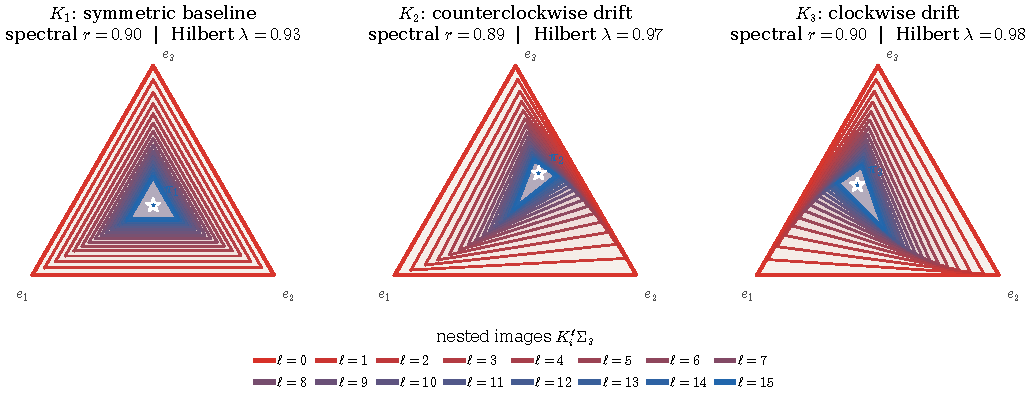
\includegraphics[width=.98\linewidth]{figures/sinkhorn-birkhoff-simplex-contraction/simplex-contraction.pdf}
\caption{\emph{Positive Markov kernels contract the three-state simplex and can simultaneously rotate its image.} Each colored polygon is $\K_i^\ell\simplex_3$: color progresses from red at $\ell=0$ to blue at $\ell=15$, and the star is the common stationary vector $\pi_i=\ones_3/3$. The isotropic kernel $\K_1$ preserves edge directions, $\K_2$ rotates an essentially homothetic triangle, and the non-normal kernel $\K_3=\K_{\mathrm{aniso}}$ both turns and strongly elongates the image because its two tangent modes contract at unequal rates. The red boundary contains zero coordinates and is only a geometric reference: positivity sends the first image into the simplex interior, where Hilbert contraction applies.}
\label{fig:sinkhorn-birkhoff-simplex-contraction}
\index{Birkhoff!contraction theorem}% strictindex
\index{Hilbert!projective metric}% strictindex
\end{figure}

The same theorem holds for positive linear maps between proper cones. Order-preserving homogeneous nonlinear maps admit related projective nonexpansiveness and contraction results, but a generic affine map is not covered because projective homogeneity is essential.
\index{positive!linear map}% strictindex

The following result, due to Franklin and Lorenz~\cite{franklin1989scaling}, applies Theorem~\ref{thm-birkhoff} to obtain global linear convergence of Sinkhorn's scaling rays.
\index{linear!convergence}% strictindex
\index{Sinkhorn!algorithm}% strictindex

\begin{thm}[Projective linear convergence of Sinkhorn]\label{thm-sinkhorn-hilbert-linear}
	Let $\vD^{(0)}>0$, define the Sinkhorn iterates by~\eqref{eq-sinkhorn}, and fix any optimal scaling pair $(\uD^\star,\vD^\star)$. For $\ell\geq1$, set
	\[
		\P^{(\ell)}
		\eqdef
		\diag(\uD^{(\ell)})\K\diag(\vD^{(\ell)}),
	\]
	and, for $\ell\geq0$, denote the row-normalized half-step by
	\[
		\P^{(\ell+1/2)}
		\eqdef
		\diag(\uD^{(\ell+1)})\K\diag(\vD^{(\ell)}).
	\]
	Writing $\la=\la(\K)$, one has
	\eql{\label{eq-convlin-sinkh}
		\Hilbert(\vD^{(\ell)},\vD^\star)
		\leq
		\la^{2\ell}\Hilbert(\vD^{(0)},\vD^\star),
		\qquad
		\Hilbert(\uD^{(\ell+1)},\uD^\star)
		\leq
		\la^{2\ell+1}\Hilbert(\vD^{(0)},\vD^\star).
	}
	Thus the scaling rays converge linearly. After fixing any continuous gauge, their representatives converge, and $\P^{(\ell)}\to\P^\star$ entrywise. The following posterior estimates use the marginal that is not yet exact at the corresponding step; the first holds for $\ell\geq1$ and the second for $\ell\geq0$:
	\eql{\label{eq-convsinkh-control}
		\Hilbert(\uD^{(\ell)},\uD^\star)
		\leq
		\frac{\Hilbert(\P^{(\ell)}\ones_m,\a)}{1-\la^2}
		\qandq
		\Hilbert(\vD^{(\ell)},\vD^\star)
		\leq
		\frac{\Hilbert((\P^{(\ell+1/2)})^\top\ones_n,\b)}{1-\la^2}.
	}
	\eqllead{Lastly,}{eq-convlin-sinkh-prim}{
		\norm{\log(\P^{(\ell)})-\log(\P^\star)}_\infty
		\leq
		\Hilbert(\uD^{(\ell)},\uD^\star)
		+
		\Hilbert(\vD^{(\ell)},\vD^\star),
	}
	where $\P^\star$ is the unique solution of~\eqref{eq-regularized-discr}.
\end{thm}

\begin{proof}
	Entrywise multiplication by a fixed positive vector and entrywise inversion are isometries of Hilbert's metric. Therefore the row map $R(\vD)=\a/(\K\vD)$ and the column map $C(\uD)=\b/(\K^\top\uD)$ are both $\la$-Lipschitz by Theorem~\ref{thm-birkhoff}. Their full-cycle compositions $C\circ R$ and $R\circ C$ are $\la^2$-contractions. Since $\vD^\star=C(R(\vD^\star))$ and $\uD^\star=R(C(\uD^\star))$, iteration gives~\eqref{eq-convlin-sinkh}.

	For any contraction $F$ with factor $q<1$ and fixed point $x^\star$, the triangle inequality gives
	\[
		d(x,x^\star)
		\leq
		d(x,Fx)+d(Fx,Fx^\star)
		\leq
		d(x,Fx)+q\,d(x,x^\star),
	\]
	hence $d(x,x^\star)\leq d(x,Fx)/(1-q)$. Apply this with $q=\la^2$ to the two full-cycle maps. The scaling identities imply
	\[
		\Hilbert(\uD^{(\ell+1)},\uD^{(\ell)})
		=
		\Hilbert(\a,\P^{(\ell)}\ones_m),
	\]
	and
	\[
		\Hilbert(\vD^{(\ell+1)},\vD^{(\ell)})
		=
		\Hilbert(\b,(\P^{(\ell+1/2)})^\top\ones_n),
	\]
	which proves~\eqref{eq-convsinkh-control}.

	Finally, write $\xi_i=\log(u_i^{(\ell)}/u_i^\star)$ and $\zeta_j=\log(v_j^{(\ell)}/v_j^\star)$. Then
	\[
		\log(\P_{i,j}^{(\ell)}/\P_{i,j}^\star)=\xi_i+\zeta_j,
		\qquad
		\operatorname{osc}(\xi\oplus\zeta)=\operatorname{osc}(\xi)+\operatorname{osc}(\zeta).
	\]
	Both plans have total mass one, so $\sum_{i,j}\P_{i,j}^\star e^{\xi_i+\zeta_j}=1$. Consequently $\min(\xi\oplus\zeta)\leq0\leq\max(\xi\oplus\zeta)$, and the sup norm of $\xi\oplus\zeta$ is bounded by its oscillation. This proves~\eqref{eq-convlin-sinkh-prim}.
\end{proof}

\paragraph{Nonlinear Sinkhorn images of the simplex.}
The preceding contraction can be visualized simultaneously for every possible scaling ray, rather than along a single initialization. Using the row and column maps from the proof, define the full-cycle map on the left scaling by
\index{Sinkhorn!full-cycle map}% strictindex
\[
	F_{\uD}(\uD)
	\eqdef
	R(C(\uD))
	=
	\a\oslash\left[\K\left(\b\oslash(\K^\top\uD)\right)\right].
\]
It is positively homogeneous, $F_{\uD}(s\uD)=sF_{\uD}(\uD)$ for $s>0$, and therefore induces the projective self-map
\[
	\widehat F_{\uD}(p)
	\eqdef
	\frac{F_{\uD}(p)}{\dotp{F_{\uD}(p)}{\ones_3}},
	\qquad p\in\simplex_3.
\]
Thus $\widehat\uD^{(\ell)}\eqdef\uD^{(\ell)}/\dotp{\uD^{(\ell)}}{\ones_3}$ follows
$\widehat\uD^{(\ell+1)}=\widehat F_{\uD}(\widehat\uD^{(\ell)})$ when $\ell$ indexes complete Sinkhorn cycles. Since $\widehat F_{\uD}$ maps $\simplex_3$ into itself, its set-valued iterates are nested:
\[
	\widehat F_{\uD}^{\,\ell+1}(\simplex_3)
	=
	\widehat F_{\uD}^{\,\ell}\!\left(\widehat F_{\uD}(\simplex_3)\right)
	\subseteq
	\widehat F_{\uD}^{\,\ell}(\simplex_3).
\]
Unlike the linear images in Figure~\ref{fig:sinkhorn-birkhoff-simplex-contraction}, these sets need not be polygons. Theorem~\ref{thm-sinkhorn-hilbert-linear} quantifies their projective shrinkage: since the first image is strictly positive,
\index{Hilbert!diameter}% strictindex
\[
	\operatorname{diam}_{\Hilbert}\!\left(\widehat F_{\uD}^{\,\ell}(\simplex_3)\right)
	\leq
	\la(\K)^{2(\ell-1)}
	\operatorname{diam}_{\Hilbert}\!\left(\widehat F_{\uD}(\simplex_3)\right),
	\qquad \ell\geq1.
\]
Figure~\ref{fig:sinkhorn-projective-scaling-simplex} reuses the three kernels $\K_i$ from Figure~\ref{fig:sinkhorn-birkhoff-simplex-contraction}, with the same uniform Sinkhorn marginals $\a=\b=\ones_3/3$ in every panel. This isolates the passage from the linear action $\K_i^\ell$ to the nonlinear balancing map $\widehat F_{\uD,i}^{\,\ell}$. The symmetric control remains aligned, $\K_2$ turns the curved images, and the unequal tangent rates of $\K_3$ additionally produce a pronounced anisotropic collapse. Here the kernels are doubly stochastic, so the normalized Sinkhorn fixed ray and stationary Markov vector both equal $\ones_3/3$; they need not coincide for general kernels and marginals.

\begin{figure}[H]
\centering
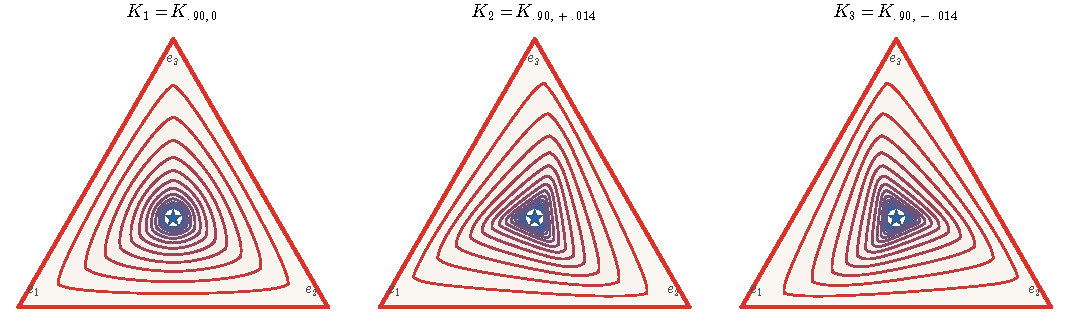
\includegraphics[width=.98\linewidth]{figures/sinkhorn-projective-scaling-simplex/scaling-contraction.pdf}
\caption{\emph{Complete Sinkhorn cycles curve, turn and contract the simplex of normalized left scalings.} Panel $i$ uses the kernel $\K_i$ identified in Figure~\ref{fig:sinkhorn-birkhoff-simplex-contraction} and the common marginals $\a=\b=\ones_3/3$. Color shows the densely sampled boundary of $\widehat F_{\uD,i}^{\,\ell}(\simplex_3)$, progressing from the red triangle at $\ell=0$ to the blue curve at $\ell=15$; the star marks $\widehat\uD_i^\star=\ones_3/3$. Coordinatewise reciprocals curve every image; $\K_2$ adds a gradual turn, whereas the non-normal $\K_3$ combines turning with a much stronger collapse across one tangent direction. Since these kernels are invertible, the projective maps are injective and the sampled curves are the actual boundaries of the nested images. The outer boundary contains zeros; the Hilbert estimate starts after one positive cycle.}
\label{fig:sinkhorn-projective-scaling-simplex}
\index{Sinkhorn!scaling}% strictindex
\index{Hilbert!projective metric}% strictindex
\end{figure}

\paragraph{Dual-potential form of the contraction.}
\index{dual!potential}% strictindex
\index{Birkhoff!contraction theorem}% strictindex

By~\eqref{eq-entropy-pd}, the KL-normalized potentials satisfy
\(
	\fD^{(\ell)}=\epsilon\log(\uD^{(\ell)}\oslash\a)
\)
and
\(
	\gD^{(\ell)}=\epsilon\log(\vD^{(\ell)}\oslash\b)
\).
The Hilbert contraction can therefore be read directly on potential classes because
\[
	\norm{\fD^{(\ell)}-\fD^\star}_V
	=
	\epsilon\Hilbert(\uD^{(\ell)},\uD^\star),
	\qquad
	\norm{\gD^{(\ell)}-\gD^\star}_V
	=
	\epsilon\Hilbert(\vD^{(\ell)},\vD^\star).
\]
Thus a complete cycle contracts both potential classes at the rate $\la(\K)^2$. Moreover, the temperature factor must be retained when passing from potentials to densities:
\eq{
	\norm{ \log \frac{\d\pi^{(\ell)}}{\d\pi^\star} }_\infty
	=
	\frac1\epsilon
	\norm{ (\fD^{(\ell)}-\fD^\star) \oplus (\gD^{(\ell)}-\gD^\star) }_\infty
	\leq
	\frac{\norm{\fD^{(\ell)}-\fD^\star}_V + \norm{\gD^{(\ell)}-\gD^\star}_V}{\epsilon}.
}
Here the last inequality uses the common mass normalization exactly as in the proof of~\eqref{eq-convlin-sinkh-prim}. For the Gibbs kernel $\K_\epsilon=e^{-\C/\epsilon}$, let $R=\max_{i,j}\C_{i,j}-\min_{i,j}\C_{i,j}$. With $\eta=\eta(\K_\epsilon)$ as in Theorem~\ref{thm-birkhoff},
\index{contraction ratio}% strictindex
\index{Gibbs!kernel}% strictindex
\[
	\la=\frac{\sqrt{\eta}-1}{\sqrt{\eta}+1}
	\leq
	\tanh(R/(2\epsilon))<1 .
\]
Indeed, every logarithmic kernel cross-ratio is bounded by $2R/\epsilon$. The posterior estimates~\eqref{eq-convsinkh-control} become
\[
	\norm{\fD^{(\ell)}-\fD^\star}_V
	\leq
	\frac{\epsilon}{1-\la^2}
	\norm{\log((\P^{(\ell)}\ones_m)\oslash\a)}_V,
\]
and
\[
	\norm{\gD^{(\ell)}-\gD^\star}_V
	\leq
	\frac{\epsilon}{1-\la^2}
	\norm{\log(((\P^{(\ell+1/2)})^\top\ones_n)\oslash\b)}_V.
\]
These are genuine posterior bounds because they use the marginal that has not yet been normalized.


%%%

The marginal violations $\norm{\P^{(\ell)}\ones_m-\a}_1$ and $\norm{(\P^{(\ell+1/2)})^\top\ones_n-\b}_1$ remain useful practical stopping criteria. At each stage one must monitor the marginal that has not just been normalized; these two residuals vanish only as the iteration approaches a common fixed point.
\index{marginal!constraint}% strictindex
Theorem~\ref{thm-sinkhorn-hilbert-linear} shows global linear convergence in projective geometry, but its worst-case rate becomes exponentially bad as $\epsilon\rightarrow0$: $1-\la(\K_\epsilon)^2$ can be of order $e^{-R/\epsilon}$. In practice, one often observes a much better local linear regime after enough iterations, and sharper continuous analyses can replace this exponential dependence by polynomial rates under additional semiconcavity or log-concavity assumptions~\cite{chizat2024sharper}.
\index{Sinkhorn!algorithm}% strictindex
%
The same Hilbert-metric mechanism extends beyond finite matrices to positive integral operators under suitable compactness and positivity assumptions.
%
An important limitation of this analysis is that it requires a uniformly bounded cost and a kernel bounded away from degeneracy; Gaussian distributions with quadratic cost therefore require a different approach.
\index{quadratic!cost}% strictindex

%%%%%%%%%%%%%%%%%%%%%%%%%%%%%%%%%%%%%%%%%%%%%%%%%%%%%%%%%%%%%%%%%%%%%%%%%%%
\section{Local Convergence Analysis and Acceleration}
\label{sec-sinkhorn-local-acceleration}
\index{Sinkhorn!local convergence}% strictindex
\index{Sinkhorn!acceleration}% strictindex

The projective analysis of Section~\ref{sec-sinkhorn-hilbert} gives an initialization-independent global rate from the kernel alone, but this robust bound can be pessimistic near the solution. Linearization reveals a more precise structure: the dual Hessian, the Jacobian of a complete Sinkhorn cycle and the curvature of the entropic semi-dual are all controlled by the same conditional-expectation operator. This operator gives the sharp local factor and motivates two accelerations: over-relaxing the alternating soft transforms, or optimizing the semi-dual after eliminating one potential.

\paragraph{Conditional operator and maximal correlation.}
\index{conditional!expectation}% strictindex
\index{maximal correlation}% strictindex

The local geometry is intrinsic to the coupling and does not depend on whether it is parameterized by potentials or scalings. Let
\(
	L_0^2(\al)\eqdef\enscond{h\in L^2(\al)}{\int h\d\al=0}
\)
and define \(L_0^2(\be)\) similarly.

\begin{defn}[Conditional coupling operator]\label{def-sinkhorn-conditional-operator}
	For a coupling $\pi\in\Couplings(\al,\be)$, let
	\(
		\pi(\d x,\d y)=\al(\d x)\pi_x(\d y)
		=\be(\d y)\pi^y(\d x)
	\)
	be its two disintegrations. Define
	\(
		T_\pi:L^2(\be)\to L^2(\al)
	\)
	and
	\(
		T_\pi^*:L^2(\al)\to L^2(\be)
	\)
	by
	\eql{\label{eq-sinkhorn-conditional-operator}
		(T_\pi k)(x)\eqdef\int_\Yy k(y)\d\pi_x(y),
		\qquad
		(T_\pi^*h)(y)\eqdef\int_\Xx h(x)\d\pi^y(x).
	}
	The centered maximal correlation of $\pi$ is
	\eql{\label{eq-sinkhorn-maximal-correlation}
		\sigma(\pi)
		\eqdef
		\sup_{\substack{k\in L_0^2(\be)\\\norm{k}_{L^2(\be)}=1}}
		\norm{T_\pi k}_{L^2(\al)}
		=
		\sup_{\substack{h\in L_0^2(\al),\,k\in L_0^2(\be)\\
		\norm{h}_{L^2(\al)}=\norm{k}_{L^2(\be)}=1}}
		\int h(x)k(y)\d\pi(x,y).
	}
	For the optimal entropic coupling $\pi_\epsilon$ of~\eqref{eq-entropic-generic}, set
	\(
		T_\epsilon\eqdef T_{\pi_\epsilon}
	\)
	and
	\(
		\sigma_\epsilon\eqdef\sigma(\pi_\epsilon).
	\)
\end{defn}

The notation $T_\pi^*$ is literal: the two operators are adjoint for the $L^2(\al)$ and $L^2(\be)$ inner products. Conditional Jensen's inequality gives $\norm{T_\pi}\leq1$, while $T_\pi1=T_\pi^*1=1$, so both operators preserve centered functions and $0\leq\sigma(\pi)\leq1$. In the discrete setting of~\eqref{eq-regularized-discr}, assuming the weights are positive, the optimizer $\P_\epsilon$ gives
\eql{\label{eq-sinkhorn-conditional-operator-discrete}
	T_\epsilon=\diag(\a)^{-1}\P_\epsilon,
	\qquad
	T_\epsilon^*=\diag(\b)^{-1}\P_\epsilon^\top,
}
where adjointness is understood in the $\a$- and $\b$-weighted Euclidean inner products. Thus $\sigma_\epsilon$ is the largest nonconstant singular value of the normalized optimal coupling.
Equivalently, it is the second singular value of
\(
	\diag(\a)^{-1/2}\P_\epsilon\diag(\b)^{-1/2}
\),
whose first singular value is one.

\paragraph{Dual Hessian and exact local rate.}
\index{dual!Hessian}% strictindex
\index{Sinkhorn!Jacobian}% strictindex

Recall that $\Dd_\epsilon$ is the continuous dual objective~\eqref{eq-dual-sinkhorn-objective}, its optimizers $(f_\epsilon,g_\epsilon)$ are unique up to the gauge $(f,g)\mapsto(f+s,g-s)$ by Proposition~\ref{prop-entropic-dual-potentials}, and Sinkhorn alternates the soft transforms~\eqref{eq-continuous-dual-sinkhorn-iteration}. The following proposition identifies the linearization of all these objects without redefining them.

\begin{prop}[Dual Hessian and local Sinkhorn rate]\label{prop-sinkhorn-local-rate}
	Assume the setting of Proposition~\ref{prop-continuous-entropic-duality}, and that differentiation under the Gibbs integrals and the stated $L^2$ Taylor expansions are valid. These requirements are automatic in finite spaces and form the local regularity hypothesis in continuous settings. For bounded directions $(h,k)$ and $(h',k')$,
	\eql{\label{eq-sinkhorn-dual-hessian-form}
		-\epsilon D^2\Dd_\epsilon(f_\epsilon,g_\epsilon)
		[(h,k),(h',k')]
		=
		\int_{\Xx\times\Yy}
		(h(x)+k(y))(h'(x)+k'(y))\d\pi_\epsilon(x,y).
	}
	Hence the Hessian form extends continuously to
	\(L^2(\al)\oplus L^2(\be)\), where the positive dual curvature operator is
	\eql{\label{eq-sinkhorn-dual-hessian-operator}
		-\nabla^2\Dd_\epsilon(f_\epsilon,g_\epsilon)
		=
		\frac1\epsilon
		\begin{pmatrix}
			\Id&T_\epsilon\\
			T_\epsilon^*&\Id
		\end{pmatrix}.
	}
	After quotienting by the gauge direction $(1,-1)$ and using the product-$L^2$ quotient norm, its spectrum is contained in
	\[
		\left[\frac{1-\sigma_\epsilon}{\epsilon},
		\frac{2}{\epsilon}\right].
	\]
	Both endpoints belong to the spectrum, although the lower one need not be an eigenvalue.
	In particular, when $\sigma_\epsilon<1$, the spectral condition number of the full dual is \(2/(1-\sigma_\epsilon)\).

	The derivatives of the two soft-transform updates~\eqref{eq-soft-c-cont-f}--\eqref{eq-soft-c-cont-g} at the optimum are
	\eql{\label{eq-sinkhorn-soft-transform-jacobians}
		D[g\mapsto g^{\bar c,\epsilon}](g_\epsilon)=-T_\epsilon,
		\qquad
		D[f\mapsto f^{c,\epsilon}](f_\epsilon)=-T_\epsilon^*.
	}
	Consequently, the Jacobian of a complete cycle
	\(g\mapsto(g^{\bar c,\epsilon})^{c,\epsilon}\)
	is $T_\epsilon^*T_\epsilon$. If the gauges are fixed so that
	\(e^{(\ell)}\eqdef g^{(\ell)}-g_\epsilon\in L_0^2(\be)\), then
	\eql{\label{eq-sinkhorn-local-error}
		e^{(\ell+1)}
		=
		T_\epsilon^*T_\epsilon e^{(\ell)}
		+
		o\!\left(\norm{e^{(\ell)}}_{L^2(\be)}\right),
		\qquad
		\limsup_{\ell\to\infty}
		\frac{\norm{e^{(\ell+1)}}_{L^2(\be)}}
		{\norm{e^{(\ell)}}_{L^2(\be)}}
		\leq\sigma_\epsilon^2.
	}
	If $\sigma_\epsilon^2$ is an isolated eigenvalue and the asymptotic error has a nonzero projection onto its eigenspace, the ratio in~\eqref{eq-sinkhorn-local-error} converges to $\sigma_\epsilon^2$.
\end{prop}

\begin{proof}
	Twice differentiating the exponential term in~\eqref{eq-dual-sinkhorn-objective} gives~\eqref{eq-sinkhorn-dual-hessian-form}; the density law~\eqref{eq-continuous-entropic-density-law} identifies its reference measure with $\pi_\epsilon$. Its two diagonal terms are the $L^2$ inner products of the marginals, and its cross term is represented by $T_\epsilon$, which proves~\eqref{eq-sinkhorn-dual-hessian-operator}.

	Each quotient class has a unique representative orthogonal to the gauge direction, hence of the form
	\(
		(h_0+m,k_0+m)
	\)
	with $h_0\in L_0^2(\al)$ and $k_0\in L_0^2(\be)$. On the centered component, Cauchy--Schwarz and~\eqref{eq-sinkhorn-maximal-correlation} give
	\[
		(1-\sigma_\epsilon)
		\bigl(\norm{h_0}_{L^2(\al)}^2+\norm{k_0}_{L^2(\be)}^2\bigr)
		\leq
		\norm{h_0}_{L^2(\al)}^2+\norm{k_0}_{L^2(\be)}^2
		+2\langle h_0,T_\epsilon k_0\rangle_{L^2(\al)}
		\leq
		(1+\sigma_\epsilon)
		\bigl(\norm{h_0}_{L^2(\al)}^2+\norm{k_0}_{L^2(\be)}^2\bigr).
	\]
	The common-constant direction $(1,1)$ has eigenvalue $2/\epsilon$, whereas $(1,-1)$ is the gauge kernel. Approximate maximizers in~\eqref{eq-sinkhorn-maximal-correlation} show that the lower spectral endpoint is $(1-\sigma_\epsilon)/\epsilon$, while the constant direction gives the upper endpoint $2/\epsilon$. This proves the condition-number formula without requiring a singular-vector basis.

	Differentiating either log-partition formula in Definition~\ref{def-continuous-soft-c-transform} produces minus the corresponding conditional expectation under $\pi_\epsilon$, proving~\eqref{eq-sinkhorn-soft-transform-jacobians}. The chain rule and a Taylor expansion then give~\eqref{eq-sinkhorn-local-error}. Since
	\(\norm{T_\epsilon^*T_\epsilon}_{L_0^2(\be)\to L_0^2(\be)}
	=\sigma_\epsilon^2\),
	the rate follows.
\end{proof}

In finite spaces, this recovers the second-singular-value description of the asymptotic matrix-scaling rate~\cite{knight2008sinkhorn,lehmann2022overrelaxation}.

The same spectral gap has a direct probabilistic interpretation. The law of total variance gives
\eql{\label{eq-sinkhorn-conditional-variance-gap}
	1-\sigma_\epsilon^2
	=
	\inf_{\substack{k\in L_0^2(\be)\\\norm{k}_{L^2(\be)}=1}}
	\int_\Xx
	\operatorname{Var}_{\pi_{\epsilon,x}}\!\bigl(k(Y)\bigr)
	\d\al(x).
}
Thus Sinkhorn slows down when the optimal conditional laws $Y|X=x$ become nearly deterministic. This is exactly what happens as $\epsilon\to0$ in a smooth Monge regime.

\begin{prop}[The global Hilbert factor controls the local rate]\label{prop-sinkhorn-hilbert-controls-local}
	In the discrete positive-kernel setting of Theorem~\ref{thm-sinkhorn-hilbert-linear}, let $\la(\K)$ be the Birkhoff contraction factor defined in Theorem~\ref{thm-birkhoff}. Then
	\eql{\label{eq-sinkhorn-hilbert-controls-local}
		\sigma_\epsilon\leq\la(\K)<1,
		\qquad
		\sigma_\epsilon^2\leq\la(\K)^2.
	}
\end{prop}
\begin{proof}
	Let $R(\vD)=\a\oslash(\K\vD)$ and $C(\uD)=\b\oslash(\K^\top\uD)$ be the row and column scaling maps used in the proof of Theorem~\ref{thm-sinkhorn-hilbert-linear}. Entrywise inversion and multiplication by a fixed positive vector are isometries of Hilbert's metric. Theorem~\ref{thm-birkhoff}, applied successively to $\K$ and $\K^\top$, therefore gives the pairwise estimate
	\[
		\Hilbert\bigl(C(R(\vD)),C(R(\widetilde\vD))\bigr)
		\leq
		\la(\K)^2\Hilbert(\vD,\widetilde\vD),
	\]
	where $\la(\K^\top)=\la(\K)$ follows directly from its cross-ratio definition. Under the logarithmic change of variables $g=\epsilon\log\vD$, Hilbert's metric becomes $\epsilon^{-1}\norm{\cdot}_V$ by~\eqref{eq-hilbert-metric}. Hence the complete dual update
	\(
		\mathcal S(g)\eqdef(g^{\bar c,\epsilon})^{c,\epsilon}
	\)
	is $\la(\K)^2$-Lipschitz for the variation norm on the quotient by constants:
	\[
		\norm{\mathcal S(g)-\mathcal S(\widetilde g)}_V
		\leq
		\la(\K)^2\norm{g-\widetilde g}_V.
	\]
	Differentiate this inequality at the fixed point $g_\epsilon$. Proposition~\ref{prop-sinkhorn-local-rate} gives
	\(D\mathcal S(g_\epsilon)=T_\epsilon^*T_\epsilon\), and therefore
	\[
		\norm{T_\epsilon^*T_\epsilon h}_V
		\leq
		\la(\K)^2\norm{h}_V
		\qquad
		\text{for every }h\in L_0^2(\be).
	\]
	In the present finite-dimensional setting, $T_\epsilon^*T_\epsilon$ is positive and self-adjoint for the $\be$-weighted inner product, and its largest eigenvalue on $L_0^2(\be)$ is $\sigma_\epsilon^2$. If $\sigma_\epsilon>0$, take a corresponding eigenvector $h_\star$. It is nonconstant, so $\norm{h_\star}_V>0$, and the preceding bound gives
	\[
		\sigma_\epsilon^2\norm{h_\star}_V
		=
		\norm{T_\epsilon^*T_\epsilon h_\star}_V
		\leq
		\la(\K)^2\norm{h_\star}_V.
	\]
	The conclusion is immediate; the case $\sigma_\epsilon=0$ is trivial.
\end{proof}

The same argument applies when the Gibbs kernel is continuous and strictly positive on compact marginal supports: the corresponding optimal coupling has a density relative to $\al\otimes\be$ that is bounded above and below, the conditional operator is compact, and the continuous Birkhoff--Hopf coefficient bounds $\sigma_\epsilon$ strictly below one.

The proposition makes the relation with the preceding section precise: maximal correlation is the sharp local quantity, whereas Birkhoff contraction supplies an input-level global upper bound. The latter can become exponentially close to one as $\epsilon\to0$. In a smooth nondegenerate Monge regime, the conditional laws have width $O(\sqrt\epsilon)$. If a uniform Laplace expansion turns the conditional-variance form in~\eqref{eq-sinkhorn-conditional-variance-gap} into $\epsilon$ times a coercive weighted Dirichlet form, then
\(
	1-\sigma_\epsilon^2\asymp\epsilon.
\)
This explains why observed local rates can be polynomially better than the universal Hilbert estimate. Related non-asymptotic continuous bounds with polynomial dependence on $\epsilon$ are proved under regularity and log-concavity hypotheses in~\cite{chizat2024sharper}; Proposition~\ref{prop-gaussian-sinkhorn-1d-rate} gives an explicit Gaussian instance of the local calculation.

\paragraph{Blockwise over-relaxation.}
\index{Sinkhorn!over-relaxation}% strictindex
\index{successive over-relaxation}% strictindex

Sinkhorn performs exact maximization in one dual block after the other. A minimal acceleration extrapolates each block toward its soft-transform maximizer~\cite{thibault2021overrelaxed,lehmann2022overrelaxation}: for $\omega>0$,
\eql{\label{eq-sinkhorn-block-overrelaxation}
	\begin{aligned}
		f^{(\ell+1)}
		&=(1-\omega)f^{(\ell)}
		+\omega(g^{(\ell)})^{\bar c,\epsilon},\\
		g^{(\ell+1)}
		&=(1-\omega)g^{(\ell)}
		+\omega(f^{(\ell+1)})^{c,\epsilon}.
	\end{aligned}
}
The choice $\omega=1$ is the original iteration~\eqref{eq-continuous-dual-sinkhorn-iteration}; $0<\omega<1$ damps the updates, while $1<\omega<2$ over-relaxes them.

\begin{prop}[Optimal local block relaxation]\label{prop-sinkhorn-optimal-overrelaxation}
	Assume the hypotheses of Proposition~\ref{prop-sinkhorn-local-rate} and $\sigma_\epsilon<1$. For every $0<\omega<2$, the iteration~\eqref{eq-sinkhorn-block-overrelaxation} is locally linearly convergent modulo the additive gauge. Its optimal relaxation parameter and corresponding asymptotic factor are
	\eql{\label{eq-sinkhorn-optimal-overrelaxation}
		\omega_\star
		=
		\frac{2}{1+\sqrt{1-\sigma_\epsilon^2}},
		\qquad
		r_\star
		=
		\omega_\star-1
		=
		\frac{1-\sqrt{1-\sigma_\epsilon^2}}
		{1+\sqrt{1-\sigma_\epsilon^2}}.
	}
	For $\omega=1$, the factor is $\sigma_\epsilon^2$, as in Proposition~\ref{prop-sinkhorn-local-rate}.
\end{prop}

\begin{proof}
	Use~\eqref{eq-sinkhorn-soft-transform-jacobians}. The polar decomposition of $T_\epsilon$ and the spectral theorem for $(T_\epsilon^*T_\epsilon)^{1/2}$ reduce the centered linearized iteration to scalar spectral values $s\in[0,\sigma_\epsilon]$; in finite dimensions these are the usual singular values. On the corresponding two-dimensional mode, one relaxed cycle has matrix
	\[
		\mathsf M_\omega(s)
		=
		\begin{pmatrix}
			1-\omega&-\omega s\\
			-\omega s(1-\omega)&1-\omega+\omega^2s^2
		\end{pmatrix},
	\]
	whose characteristic polynomial is
	\[
		z^2-\left(2(1-\omega)+\omega^2s^2\right)z+(1-\omega)^2.
	\]
	The supremum of the root moduli is reached, or approached, as $s\to\sigma_\epsilon$. The two roots of this limiting mode have equal modulus precisely when
	\(\omega^2\sigma_\epsilon^2=4(\omega-1)\).
	The smaller solution is $\omega_\star$ in~\eqref{eq-sinkhorn-optimal-overrelaxation}; at this value both root moduli equal $\omega_\star-1$. Below this threshold the dominant real root decreases with $\omega$, while above it the conjugate-root modulus $\omega-1$ increases. This proves optimality and local convergence for $0<\omega<2$.
	The nongauge constant mode has factor $(1-\omega)^2$ and never dominates these centered modes.
\end{proof}

Set $\delta_\epsilon=1-\sigma_\epsilon^2$. When $\delta_\epsilon$ is small, the exact expression in~\eqref{eq-sinkhorn-optimal-overrelaxation} gives the complete-cycle factor
\[
	r_\star
	=
	\frac{1-\sqrt{\delta_\epsilon}}{1+\sqrt{\delta_\epsilon}}
	=
	1-2\sqrt{\delta_\epsilon}
	+2\delta_\epsilon
	O(\delta_\epsilon^{3/2}),
\]
instead of $\sigma_\epsilon^2=1-\delta_\epsilon$ for ordinary Sinkhorn. The coefficient two is specific to measuring one complete two-block cycle. Per half-step, the corresponding factor is
\(
	\sqrt{r_\star}=1-\sqrt{\delta_\epsilon}+O(\delta_\epsilon)
\).
This is a local prescription. In the finite positive-kernel setting, the Hilbert estimate used in Theorem~\ref{thm-sinkhorn-hilbert-linear} yields global convergence of the relaxed iteration for the conservative range~\cite{lehmann2022overrelaxation}
\(
	0<\omega<2/(1+\la(\K))
\);
larger choices require the adaptive safeguards analyzed in~\cite{thibault2021overrelaxed,lehmann2022overrelaxation}.

Figure~\ref{fig:sinkhorn-overrelaxation} compares this local prediction with nonlinear iterations. A common ordinary-Sinkhorn warm start places all five runs in the local regime before their relaxation parameters are changed.

\begin{figure}[H]
\centering

\includegraphics[width=.99\linewidth]{figures/sinkhorn-overrelaxation/overview.pdf}
\caption{\emph{Blockwise over-relaxation accelerates local Sinkhorn convergence.} Left: the entropic coupling at $\epsilon=10^{-2}$; only entries larger than $35\%$ of the maximal mass are drawn, with segment widths proportional to their masses. Middle: after $300$ common ordinary-Sinkhorn warm-up cycles, the residual $r_\ell\eqdef\frac12(\|\P^{(\ell)}\ones-\a\|_1+\|(\P^{(\ell)})^\top\ones-\b\|_1)$ is shown for $\omega\in\{0.5,1,\omega_\star,(\omega_\star+2)/2,1.97\}$; $\omega=1$ is ordinary Sinkhorn, and curves stop at numerical roundoff. Right: the continuous curve is the theoretical one-cycle gain $1-r_{\rm loc}(\omega)$, where $r_{\rm loc}(\omega)$ is the spectral radius of the centered linearization obtained from the maximal correlation $\sigma_\epsilon\simeq0.993$ of the limiting coupling. Filled circles mark this prediction at the five displayed parameters; crosses show the empirical gains $1-\widehat r_{\rm marg}(\omega)$ obtained by fitting $\log r_\ell$ affinely over the final $80$ available iterates above the numerical floor. Equation~\eqref{eq-sinkhorn-optimal-overrelaxation} gives $\omega_\star\simeq1.79$.}
\label{fig:sinkhorn-overrelaxation}
\end{figure}

\paragraph{Entropic semi-dual and variable projection.}
\index{semi-dual!entropic}% strictindex
\index{variable projection}% strictindex

The hard semi-dual \(\Ee_0\) in~\eqref{eq-semi-dual} eliminates one potential from the full dual \(\Dd_0\). At positive temperature, the full dual is \(\Dd_\epsilon\) from~\eqref{eq-dual-sinkhorn-objective}, and the soft \(\bar c\)-transform \(g^{\bar c,\epsilon}\) is defined by~\eqref{eq-soft-c-cont-g}. Applying the same partial maximization gives the entropic semi-dual
\eql{\label{eq-entropic-semidual-local}
	\Ee_\epsilon(g)
	\eqdef
	\Dd_\epsilon(g^{\bar c,\epsilon},g)
	=
	\int_\Xx g^{\bar c,\epsilon}\d\al
	+
	\int_\Yy g\d\be.
}
The exponential term disappears in the last equality because the first marginal is normalized by the soft transform. This exact block elimination is an instance of variable projection (VarPro)~\cite{golub1973variableprojection,golub2003variableprojection}. The VarPro principle is to optimize out one block of variables exactly whenever its conditional optimizer is available at an acceptable cost. At the level of optimization geometry, this reduction is always favorable: it removes variables and cannot worsen the local spectral conditioning, as quantified below. Its computational value depends on the cost of the inner solve.

VarPro was introduced for separable nonlinear least-squares problems. A representative later application is the training of a two-layer neural network with nonlinear hidden parameters $\theta$, feature matrix $\Phi_\theta(X)$ and linear output weights $A$:
\[
	\min_{\theta,A}\frac12\|A\Phi_\theta(X)-Y\|_{\rm F}^2.
\]
For fixed $\theta$, optimizing $A$ is a convex linear least-squares problem that can be solved by QR or SVD, or through its normal-equation linear system, and is therefore practical for moderate-size problems; one then optimizes the reduced, generally nonconvex, objective in $\theta$~\cite{kim2008variableprojection}. The present use is structurally different. The Sinkhorn dual $\Dd_\epsilon(f,g)$ is jointly concave in $(f,g)$, or equivalently $-\Dd_\epsilon$ is jointly convex, and the eliminated block does not require a least-squares solve: its exact maximizer is the closed-form soft transform $f=g^{\bar c,\epsilon}$.

For a potential $g$, let $\pi_g$ be the Gibbs measure obtained from the density law~\eqref{eq-continuous-entropic-density-law} by replacing $(f_\epsilon,g_\epsilon)$ with $(g^{\bar c,\epsilon},g)$. Write
\(
	\pi_g(\d x,\d y)=\al(\d x)\pi_{g,x}(\d y)
\)
and denote its second marginal by $\be_g$. The first marginal is exactly $\al$ by construction.

\begin{prop}[Semi-dual curvature and conditioning]\label{prop-sinkhorn-semidual-curvature}
	For bounded directions $k,k'$,
	\eql{\label{eq-entropic-semidual-derivatives}
		D\Ee_\epsilon(g)[k]
		=
		\int_\Yy k\d(\be-\be_g),
		\qquad
		D^2\Ee_\epsilon(g)[k,k']
		=
		-\frac1\epsilon
		\int_\Xx
		\operatorname{Cov}_{\pi_{g,x}}\!\bigl(k(Y),k'(Y)\bigr)
		\d\al(x).
	}
	At $g=g_\epsilon$, its positive curvature on $L_0^2(\be)$ is
	\eql{\label{eq-entropic-semidual-hessian}
		-\nabla^2\Ee_\epsilon(g_\epsilon)
		=
		\frac1\epsilon(\Id-T_\epsilon^*T_\epsilon),
		\qquad
		\frac{1-\sigma_\epsilon^2}{\epsilon}\Id
		\preceq
		-\nabla^2\Ee_\epsilon(g_\epsilon)
		\preceq
		\frac1\epsilon\Id.
	}
	Hence its spectral condition number is at most
	\(
		1/(1-\sigma_\epsilon^2)
	\).
	Gradient ascent on the local quadratic model, with the minimax constant step based only on these spectral bounds,
	\(
		2\epsilon/(2-\sigma_\epsilon^2)
	\),
	has factor
	\eql{\label{eq-entropic-semidual-gradient-rate}
		r_{\rm grad}
		\leq
		\frac{\sigma_\epsilon^2}{2-\sigma_\epsilon^2}.
	}
\end{prop}

\begin{proof}
	The envelope theorem gives the first derivative in~\eqref{eq-entropic-semidual-derivatives}. Differentiating the normalized conditional Gibbs law gives the covariance formula. At the optimum, total covariance yields
	\[
		\int_\Xx
		\operatorname{Cov}_{\pi_{\epsilon,x}}(k(Y),k'(Y))
		\d\al(x)
		=
		\int_\Yy kk'\d\be
		-
		\int_\Xx(T_\epsilon k)(T_\epsilon k')\d\al,
	\]
	which is~\eqref{eq-entropic-semidual-hessian}. Equivalently, this operator is the Schur complement of the first identity block in~\eqref{eq-sinkhorn-dual-hessian-operator}. Its spectrum on centered functions lies in
	\(
		[(1-\sigma_\epsilon^2)/\epsilon,1/\epsilon]
	\).
	The standard optimal-step formula for a quadratic with spectral interval $[\alpha,L]$ gives factor $(L-\alpha)/(L+\alpha)$, which here is~\eqref{eq-entropic-semidual-gradient-rate}.
\end{proof}

Variable projection cannot worsen local spectral conditioning~\cite{golub1973variableprojection,golub2003variableprojection}: the Schur-complement quadratic form is the minimum of the full quadratic form over the eliminated block, so its smallest eigenvalue cannot decrease and its largest eigenvalue cannot increase. Here the gain has a simple explicit bound. The full-dual condition number from Proposition~\ref{prop-sinkhorn-local-rate} is $2/(1-\sigma_\epsilon)$, whereas the semi-dual condition number is at most $1/(1-\sigma_\epsilon^2)$; this upper bound is smaller by the factor $2(1+\sigma_\epsilon)$. This comparison is available because both diagonal blocks in~\eqref{eq-sinkhorn-dual-hessian-operator} are identities.

There is also a useful algorithmic comparison. Writing
\(
	r_g\eqdef\d\be_g/\d\be
\)
and using the two soft transforms gives
\eql{\label{eq-sinkhorn-semidual-gradient-comparison}
	r_g
	=
	\exp\!\left(
		\frac{g-(g^{\bar c,\epsilon})^{c,\epsilon}}{\epsilon}
	\right),
	\qquad
	\nabla\Ee_\epsilon(g)=1-r_g.
}
Here the gradient is the Riesz gradient for the $L^2(\be)$ inner product.
Therefore one ordinary Sinkhorn cycle satisfies
\[
	(g^{\bar c,\epsilon})^{c,\epsilon}-g
	=
	-\epsilon\log r_g
	=
	\epsilon\nabla\Ee_\epsilon(g)
	+
	o\!\left(\norm{g-g_\epsilon}_{L^2(\be)}\right).
\]
Sinkhorn is thus locally semi-dual gradient ascent with step $\epsilon$, although the two nonlinear algorithms are not globally identical. Quasi-Newton methods instead learn an approximation of
\(
	\epsilon(\Id-T_\epsilon^*T_\epsilon)^{-1}
\)
from successive gradients. This explains the effectiveness of BFGS and L-BFGS on regularized semi-duals~\cite{2016-Cuturi-siims,cuturi2018semidual,nocedal}: they reuse curvature information, at the cost of storing curvature pairs and, typically, extra evaluations during line search. Stochastic first-order methods instead exploit the same semi-dual gradient formula using sampled marginals~\cite{genevay2016stochastic}.

%%%%%%%%%%%%%%%%%%%%%%%%%%%%%%%%%%%%%%%%%%%%%%%%%%%%%%%%%%%%%%%%%%%%%%%%%%%
\section{Entropic Optimal Transport between Gaussians}
\index{Gaussian!Sinkhorn}% strictindex
\label{sec-gaussian-sinkhorn}

Gaussian marginals provide an explicit finite-dimensional model of Sinkhorn's behavior. The soft $c$-transform preserves quadratic potentials, the optimal entropic coupling is Gaussian, and the value can be written with matrix square roots~\cite{janati2020gaussian}. This is the entropic counterpart of the Gaussian $\Wass_2$ formula in Proposition~\ref{prop-gaussian-w2-bures}.
\index{matrix!square root}% strictindex
\index{soft!c-transform}% strictindex
\index{quadratic!potential}% strictindex
\index{Gaussian!marginals}% strictindex

\begin{prop}[Quadratic closure of Sinkhorn iterates]\label{prop-gaussian-sinkhorn-closure}
\index{quadratic!closure}% strictindex
\index{Sinkhorn!iteration}% strictindex
	Let $\be=\Gaussian(\mean_\be,\cov_\be)$ on $\RR^d$ and take $c(x,y)=\norm{x-y}^2$. If $g(y)$ is a quadratic polynomial such that the Gaussian integral below is finite, then the soft transform
\index{soft!transform}% strictindex
	\[
		f(x)
		=
		-\epsilon\log
		\int
		\exp\!\left(\frac{g(y)-\norm{x-y}^2}{\epsilon}\right)
		\d\be(y)
	\]
	is a quadratic polynomial in $x$. In particular, starting Sinkhorn from $g_0=0$ gives
	\[
		f_1(x)
		=
		\frac{\epsilon}{2}
		\log\det\!\left(\Id+\frac{2\cov_\be}{\epsilon}\right)
		+
		\epsilon
		\dotp{x-\mean_\be}{(\epsilon\Id+2\cov_\be)^{-1}(x-\mean_\be)}.
	\]
\end{prop}

\begin{proof}
	The exponent is the sum of a quadratic polynomial in $y$ and the logarithm of the Gaussian density of $\be$. Completing the square in $y$ evaluates the integral as a positive constant times the exponential of a quadratic polynomial in $x$. Taking $-\epsilon\log$ therefore gives a quadratic polynomial.

	For $g_0=0$, let $Y\sim\be$. The Gaussian identity
	\[
		\EE\exp\!\left(-\frac{\norm{x-Y}^2}{\epsilon}\right)
		=
		\det\!\left(\Id+\frac{2\cov_\be}{\epsilon}\right)^{-1/2}
		\exp\!\left(
			-\dotp{x-\mean_\be}{(\epsilon\Id+2\cov_\be)^{-1}(x-\mean_\be)}
		\right)
	\]
	gives the displayed expression.
\end{proof}

\begin{prop}[Balanced entropic OT between Gaussians]\label{prop-gaussian-sinkhorn-closed-form}
\index{entropic!OT}% strictindex
\index{Gaussian!Sinkhorn}% strictindex
	Let $\al=\Gaussian(\mean_\al,\cov_\al)$ and $\be=\Gaussian(\mean_\be,\cov_\be)$ with positive-definite covariances, and let
	\[
		\cov_\al^{1/2}\cov_\be^{1/2}
		=
		U\diag(\sigma_i)V^\top
	\]
	be a singular-value decomposition. For the balanced objective
	\[
		\min_{\pi\in\Couplings(\al,\be)}
		\int\norm{x-y}^2\d\pi(x,y)
		+
		\epsilon\KL(\pi|\al\otimes\be),
	\]
	the optimizer is Gaussian with cross-covariance
	\[
		K_\epsilon
		=
		\cov_\al^{1/2}
		U\diag(s_i)V^\top
		\cov_\be^{1/2},
		\qquad
		s_i
		=
		\frac{\sqrt{\epsilon^2+16\sigma_i^2}-\epsilon}{4\sigma_i}.
	\]
	The optimal value is
	\[
		\norm{\mean_\al-\mean_\be}^2
		+
		\tr(\cov_\al)+\tr(\cov_\be)
		+
		\sum_i
		\left(
			-2\sigma_i s_i
			-\frac{\epsilon}{2}\log(1-s_i^2)
		\right).
	\]
	As $\epsilon\downarrow0$, $s_i\to1$ and the full covariance contribution, including the two trace terms, converges to $\Bb(\cov_\al,\cov_\be)^2$.
\end{prop}

\begin{proof}
	Let $(X,Y)$ be any coupling with finite second moments and cross-covariance
	\(K=\EE\big[(X-\mean_\al)(Y-\mean_\be)^\top\big]\).
	Replacing $(X,Y)$ by the Gaussian vector with the same mean and covariance leaves the quadratic cost unchanged. Since the marginals are fixed,
\index{quadratic!cost}% strictindex
	\[
		\KL(\pi|\al\otimes\be)
		=
		-h(X,Y)+h(\al)+h(\be),
	\]
	where $h$ denotes differential entropy when it is finite. Among laws with a fixed covariance, the Gaussian maximizes entropy; if the entropy is not finite, the relative entropy is already $+\infty$. Thus the Gaussian replacement cannot increase the objective, and it is enough to optimize over Gaussian couplings.
\index{relative!entropy}% strictindex

	Any such coupling has covariance
	\[
		\begin{pmatrix}
			\cov_\al & K\\
			K^\top & \cov_\be
		\end{pmatrix}.
	\]
	Write $K=\cov_\al^{1/2}S\cov_\be^{1/2}$. The block covariance constraint is equivalent to the singular values of $S$ being at most one, and finite entropy forces them to be strictly smaller than one. The cost depends on $K$ through
	\[
		\norm{\mean_\al-\mean_\be}^2+\tr(\cov_\al)+\tr(\cov_\be)-2\tr(K),
	\]
	while
	\[
		\KL(\pi|\al\otimes\be)
		=
		-\frac12\log\det(\Id-SS^\top).
	\]
	By von Neumann's trace inequality, the minimizer aligns $S$ with the singular vectors of $\cov_\al^{1/2}\cov_\be^{1/2}$, so $S=U\diag(s_i)V^\top$. The problem separates into scalar minimizations
	\[
		\min_{0\leq s<1}
		-2\sigma_i s-\frac{\epsilon}{2}\log(1-s^2).
	\]
	The first-order condition is $2\sigma_i=\epsilon s/(1-s^2)$, whose positive solution is the displayed $s_i$. Substitution gives the value formula. Since $s_i\to1$ and $\epsilon\log(1-s_i^2)\to0$ as $\epsilon\downarrow0$, the spectral sum converges to $-2\sum_i\sigma_i$. The identity
	\[
		\sum_i\sigma_i
		=
		\tr\!\left((\cov_\al^{1/2}\cov_\be\cov_\al^{1/2})^{1/2}\right)
	\]
	then gives the Bures--Wasserstein covariance contribution.
\index{Bures!Wasserstein geometry}% strictindex
\end{proof}

\begin{cor}[Gaussian Sinkhorn divergence and smoothed Bures term]\label{cor-gaussian-sinkhorn-divergence}
\index{Bures!smoothed term}% strictindex
\index{Sinkhorn!divergence}% strictindex
\index{Gaussian!Sinkhorn divergence}% strictindex
\index{Gaussian!Sinkhorn}% strictindex
	Let $\al=\Gaussian(\mean_\al,\cov_\al)$ and $\be=\Gaussian(\mean_\be,\cov_\be)$ have positive-definite covariances. For $r>0$, define
	\[
		\tau_\epsilon(r)
		\eqdef
		\frac{\sqrt{\epsilon^2+16r^2}-\epsilon}{4r},
		\qquad
		\psi_\epsilon(r)
		\eqdef
		-2r\,\tau_\epsilon(r)
		-\frac{\epsilon}{2}\log\bigl(1-\tau_\epsilon(r)^2\bigr).
	\]
	If $\sigma_i(\Sigma,\Lambda)$ denotes the singular values of $\Sigma^{1/2}\Lambda^{1/2}$ and $\lambda_i(\Sigma)$ the eigenvalues of $\Sigma$, then the debiased Sinkhorn divergence~\eqref{eq-sinkhorn-divergence} is
\index{Sinkhorn!divergence}% strictindex
	\[
		\bar\MK_{\norm{\cdot-\cdot}^2}^{\epsilon}(\al,\be)
		=
		\norm{\mean_\al-\mean_\be}^2
		+
		\Bb_\epsilon(\cov_\al,\cov_\be)^2,
	\]
	where the Gaussian covariance contribution is the debiased smoothed Bures term
\index{Gaussian!covariance}% strictindex
\index{Bures!smoothed term}% strictindex
	\[
		\Bb_\epsilon(\Sigma,\Lambda)^2
		\eqdef
		\sum_i \psi_\epsilon\bigl(\sigma_i(\Sigma,\Lambda)\bigr)
		-\frac12\sum_i\psi_\epsilon\bigl(\lambda_i(\Sigma)\bigr)
		-\frac12\sum_i\psi_\epsilon\bigl(\lambda_i(\Lambda)\bigr).
	\]
	Moreover $\Bb_\epsilon(\Sigma,\Lambda)^2\to\Bb(\Sigma,\Lambda)^2$ as $\epsilon\downarrow0$, where $\Bb$ is the Bures--Wasserstein metric of Proposition~\ref{prop-gaussian-w2-bures}.
\index{Bures!Wasserstein geometry}% strictindex
\end{cor}

\begin{proof}
	Proposition~\ref{prop-gaussian-sinkhorn-closed-form} writes the raw entropic value as the squared mean displacement plus trace terms and a spectral sum. With the notation above, the spectral part is exactly $\sum_i\psi_\epsilon(\sigma_i(\cov_\al,\cov_\be))$. Applying the same formula to the self-costs $(\al,\al)$ and $(\be,\be)$ replaces these singular values by the eigenvalues of $\cov_\al$ and $\cov_\be$. In the polarization formula~\eqref{eq-sinkhorn-divergence}, the trace terms cancel:
\index{Sinkhorn!divergence}% strictindex
	\[
		\tr\cov_\al+\tr\cov_\be
		-\frac12(2\tr\cov_\al)
		-\frac12(2\tr\cov_\be)=0,
	\]
	while the polarization of the squared mean terms leaves exactly $\norm{\mean_\al-\mean_\be}^2$. This gives the displayed formula. Since $\tau_\epsilon(r)\to1$ and $\epsilon\log(1-\tau_\epsilon(r)^2)\to0$, one has $\psi_\epsilon(r)\to-2r$. The limit is therefore
	\[
		\tr\Sigma+\tr\Lambda
		-2\sum_i\sigma_i(\Sigma,\Lambda)
		=
		\Bb(\Sigma,\Lambda)^2,
	\]
	which is the Bures formula~\eqref{eq-bure-defn}.
\end{proof}

\begin{prop}[One-dimensional Gaussian Sinkhorn rate]\label{prop-gaussian-sinkhorn-1d-rate}
\index{Gaussian!Sinkhorn}% strictindex
	Consider $\al=\be=\Gaussian(0,1)$ on $\RR$ with $c(x,y)=(x-y)^2$. If a dual potential has the form $g_q(y)=q y^2+\mathrm{cst}$, then one soft transform has quadratic coefficient
\index{dual!potential}% strictindex
\index{soft!transform}% strictindex
	\[
		\mathsf Q_\epsilon(q)
		=
		1-\frac{1}{1-q+\epsilon/2},
		\qquad q<1+\epsilon/2,
	\]
	and one full Sinkhorn cycle acts as $q\mapsto \mathsf Q_\epsilon(\mathsf Q_\epsilon(q))$. The fixed point $q_\star=\mathsf Q_\epsilon(q_\star)$ is determined by
	\[
		A_\star^2-\frac{\epsilon}{2}A_\star-1=0,
		\qquad
		A_\star\eqdef 1-q_\star+\frac{\epsilon}{2}
		=
		\frac{\epsilon+\sqrt{\epsilon^2+16}}{4}.
	\]
	The optimal Gaussian coupling of Proposition~\ref{prop-gaussian-sinkhorn-closed-form} has correlation
	\(
		s_\epsilon=A_\star^{-1}
	\).
	Hence the maximal correlation in Definition~\ref{def-sinkhorn-conditional-operator} is $\sigma_\epsilon=s_\epsilon$, and the exact local $L^2$ factor is $A_\star^{-2}$. The quadratic-potential mode contracts faster, with factor
	\[
		\rho_\epsilon=A_\star^{-4}
		=
		\left(\frac{4}{\epsilon+\sqrt{\epsilon^2+16}}\right)^4 .
	\]
\end{prop}

\begin{proof}
	Completing the square in
	\[
		\int
		\exp\!\left(\frac{q y^2-(x-y)^2}{\epsilon}\right)
		\d\Gaussian(0,1)(y)
	\]
	gives the coefficient $\mathsf Q_\epsilon(q)$. The fixed-point equation $q_\star=1-1/A_\star$, together with $q_\star=1+\epsilon/2-A_\star$, gives
	\(A_\star^2-\frac{\epsilon}{2}A_\star-1=0\).
	The positive solution is the displayed $A_\star$. Since
	\(\mathsf Q_\epsilon'(q)=-\frac{1}{(1-q+\epsilon/2)^2}\),
	the derivative of the full-cycle map at the fixed point is $\mathsf Q_\epsilon'(q_\star)^2=A_\star^{-4}$. The correlation formula is the one-dimensional specialization of Proposition~\ref{prop-gaussian-sinkhorn-closed-form}. Conditional expectation under a correlated Gaussian diagonalizes in the Hermite basis, with largest nonconstant singular value $s_\epsilon$; Proposition~\ref{prop-sinkhorn-local-rate} then gives the full factor $s_\epsilon^2=A_\star^{-2}$.
\end{proof}

This calculation illustrates the general Gaussian convergence picture of Chizat, Delalande and Va\v{s}kevi\v{c}ius~\cite{chizat2024sharper}: the rate improves when $\epsilon$ is large or the covariance scales overlap well, and deteriorates in the small-temperature limit where the entropic coupling approaches a deterministic Brenier map.
\index{Brenier!map}% strictindex


%%%%%%%%%%%%%%%%%%%%%%%%%%%%%%%%%%%%%%%%%%%%%%%%%%%%%%%%%%%%%%%%%%%%%%%%%%%

%%%%%%%%%%%%%%%%%%%%%%%%%%%%%%%%%%%%%%%%%%%%%%%%%%%%%%%%%%%%%%%%%%%%%%%%%%%
\section{Continuous \texorpdfstring{$\varepsilon$}{epsilon}-Sinkhorn Flow}\label{sec-continuous-epsilon-sinkhorn}
\index{Sinkhorn!continuous flow}% strictindex
\index{parabolic optimal transport}% strictindex

This section studies a simultaneous high-resolution, many-iteration limit of Sinkhorn. It is not the continuous-time interpolation of a fixed-temperature algorithm: the grid is refined while the temperature and the fictitious time step both vanish as $1/k$.

\paragraph{Parabolic Monge--Ampere limit.}
\index{Monge-Ampere@Monge--Amp\`ere!parabolic equation}% strictindex
The previous arguments view Sinkhorn as a discrete fixed-point iteration. A complementary picture, developed by Berman~\cite{berman2017sinkhorn}, considers the quadratic torus cost $c(x,y)=d_{\TT^d}(x,y)^2/2$, discretizes both marginals on a grid of mesh $1/k$, sets the entropic temperature to $\epsilon_k=1/k$, and assigns the same duration $\Delta t=1/k$ to each Sinkhorn update. The $\ell$-th log-potential is therefore observed at time $t=\ell/k$. In this coupled limit, the iterates converge to a fully nonlinear parabolic flow whose stationary equation is the Monge--Ampere equation for the optimal map. This connects matrix scaling with real and complex Monge--Ampere geometry.
\index{Monge-Ampere@Monge--Amp\`ere!equation}% strictindex
\index{Monge-Ampere@Monge--Amp\`ere!geometric equation}% strictindex

\begin{defn}[Continuous \texorpdfstring{$\varepsilon$}{epsilon}-Sinkhorn flow]\label{def-continuous-epsilon-sinkhorn}
\index{Sinkhorn!continuous flow}% strictindex
	Let $\al$ and $\be$ be probability measures on the unit-volume flat torus $\TT^d$ with smooth positive densities $\density{\al}=e^{-F}$ and $\density{\be}=e^{-G}$. For the cost $c(x,y)=d_{\TT^d}(x,y)^2/2$, a gauge-fixed potential $u_t:\TT^d\to\RR$, with $\int_{\TT^d}u_t\d x=0$, follows the continuous \(\varepsilon\)-Sinkhorn flow if
	\[
		\partial_t u_t(x)
		=
		\log\det\big(\Id+\nabla^2 u_t(x)\big)
		-G\big(x+\nabla u_t(x)\big)+F(x)-\bar r_t,
		\tag{CES}
	\]
	where $x+\nabla u_t(x)$ is understood modulo $\ZZ^d$, $\Id+\nabla^2u_t\succ0$, and $\bar r_t$ is the unique scalar preserving the mean-zero gauge.
\index{gauge fixing}% strictindex
\index{Sinkhorn!potential}% strictindex
\end{defn}

Explicitly,
\[
	\bar r_t
	=
	\int_{\TT^d}
	\Big[
	\log\det\big(\Id+\nabla^2 u_t(x)\big)
	-G\big(x+\nabla u_t(x)\big)+F(x)
	\Big]\d x .
\]
Its subtraction fixes the additive constant of the potential. The following operators make the discrete scaling behind this equation explicit. Let $\al^{[k]}$ and $\be^{[k]}$ be the positive grid discretizations of $\al$ and $\be$, and define
\[
	v_k[u](y)
	\eqdef
	\frac1k\log\int_{\TT^d}
	e^{-k(c(x,y)+u(x))}\d\al^{[k]}(x),
\]
followed by the double log-Sinkhorn operator
\[
	(S_k u)(x)
	\eqdef
	\frac1k\log\int_{\TT^d}
	e^{-k(c(x,y)+v_k[u](y))}\d\be^{[k]}(y).
\]
Its multiplicative increment is
\eql{\label{eq-continuous-sinkhorn-rho}
	\rho_{k,u}(x)
	\eqdef
	e^{k(S_k u(x)-u(x))}
	=
	e^{-ku(x)}
	\int_{\TT^d}
	\frac{e^{-kc(x,y)}}{
		\int_{\TT^d}e^{-k(c(x',y)+u(x'))}\d\al^{[k]}(x')}
		\d\be^{[k]}(y).
}
The normalized update is $u^{[k],(\ell+1)}=S_k u^{[k],(\ell)}-\int_{\TT^d}S_k u^{[k],(\ell)}\d x$.

\begin{prop}[Scaled log-Sinkhorn limit]\label{prop-scaled-log-sinkhorn-limit}
\index{Sinkhorn!continuous limit}% strictindex
\index{Laplace method}% strictindex
	Let $\epsilon_k=1/k$, let $\al^{[k]},\be^{[k]}$ be the regular-grid density discretizations above, and generate the mean-zero iterates with the normalized operator $S_k$. Define $u^{[k]}(t)\eqdef u^{[k],(\lfloor kt\rfloor)}$. Assume that, on every compact time interval, $u^{[k]}(t)$ converges smoothly to $u_t$, that $\Id+\nabla^2u_t\succ0$, and that the Laplace expansion below is uniform along the sequence. Then $u_t$ solves the continuous \(\varepsilon\)-Sinkhorn flow~\textup{(CES)}.
\index{Sinkhorn!continuous flow}% strictindex
\end{prop}

\begin{proof}
	By~\eqref{eq-continuous-sinkhorn-rho}, the normalized update satisfies
	\[
		u^{[k],(\ell+1)}-u^{[k],(\ell)}
		=
		k^{-1}
		\left[
		\log\rho_{k,u^{[k],(\ell)}}-
		\int_{\TT^d}\log\rho_{k,u^{[k],(\ell)}}\d x
		\right],
	\]
	where the subtraction enforces the mean-zero gauge. Berman's discrete Laplace estimate gives
	\[
		\rho_{k,u}(x)
		=
		\det(\Id+\nabla^2u(x))
		e^{F(x)-G(x+\nabla u(x))}
		\big(1+O(k^{-1})\big),
	\]
	uniformly for the smooth potentials under consideration. Taking logarithms gives
	\[
		\log\rho_{k,u}(x)
		=
		\log\det(\Id+\nabla^2u(x))
		-G(x+\nabla u(x))+F(x)+O(k^{-1}).
	\]
	Dividing the increment by the time step $1/k$, passing to the smooth limit $u^{[k]}(t)\to u_t$, and keeping the mean-zero normalization gives exactly~\textup{(CES)}.
\end{proof}

The word ``epsilon'' therefore refers to the vanishing entropic temperature before this rescaling; no explicit $\epsilon$ remains in the normalized limiting PDE. The equation is a real parabolic Monge--Ampere equation. Its K\"ahler analogue is the parabolic complex Monge--Ampere equation, which explains the link with the geometric Monge--Ampere literature emphasized by Berman.
\index{soft!c-transform}% strictindex
\index{Monge-Ampere@Monge--Amp\`ere!complex equation}% strictindex
\index{entropic!temperature}% strictindex
\index{Laplace method}% strictindex

\begin{prop}[Stationary continuous Sinkhorn potentials]\label{prop-continuous-sinkhorn-stationary}
\index{stationary potential}% strictindex
	Assume that a smooth stationary solution of~\textup{(CES)} satisfies $\Id+\nabla^2u\succ0$, and define $T(x)=x+\nabla u(x)$ modulo $\ZZ^d$. Then $T_\sharp\al=\be$. Conversely, any smooth map of this form satisfying $\Id+\nabla^2u\succ0$ and $T_\sharp\al=\be$ solves the stationary equation, up to the additive gauge of $u$.
\end{prop}

\begin{proof}
	At stationarity, the bracket in~\textup{(CES)} is a constant $c$:
	\[
		\log\det\big(\Id+\nabla^2u(x)\big)-G(T(x))+F(x)=c.
	\]
	Exponentiating, and using $\nabla T=\Id+\nabla^2u$, gives
	\[
		e^{-G(T(x))}\det(\nabla T(x))=e^{-F(x)}e^c.
	\]
	Because $T$ is homotopic to the identity and $\Id+\nabla^2u\succ0$, it is an orientation-preserving local diffeomorphism of degree one; hence it is a diffeomorphism of the torus. Since $\al$ and $\be$ have total mass one, integration and the change-of-variables formula give $e^c=1$. The same identity then becomes precisely the Jacobian equation for $T_\sharp(e^{-F}\d x)=e^{-G}\d x$. The converse follows by reversing this argument.
\index{Jacobian equation}% strictindex
\index{change of variables formula}% strictindex
\end{proof}

\paragraph{Gaussian closure.}
\index{Gaussian!closure}% strictindex
Gaussian marginals give a finite-dimensional test case for the continuous flow. The theorem above is stated on the flat torus, but the same local Laplace calculation can be read formally on \(\RR^d\) for confining Gaussian densities. Write
\(\al=\Gaussian(\mean_\al,\cov_\al)\) and \(\be=\Gaussian(\mean_\be,\cov_\be)\), and restrict the potential to the quadratic ansatz for which
\[
	T_t(x)\eqdef x+\nabla u_t(x)
	=
	q_t+B_t(x-\mean_\al),
	\qquad B_t\in\mathbb S_{++}^d .
\]
Taking the spatial gradient of~\textup{(CES)} removes the additive gauge. Since
\[
	F(x)=\frac12\dotp{x-\mean_\al}{\cov_\al^{-1}(x-\mean_\al)}+\mathrm{cst},
	\qquad
	G(y)=\frac12\dotp{y-\mean_\be}{\cov_\be^{-1}(y-\mean_\be)}+\mathrm{cst},
\]
coefficient matching in the identity \(\partial_tT_t=\nabla\partial_tu_t\) gives
\[
	\dot B_t=\cov_\al^{-1}-B_t\cov_\be^{-1}B_t,
	\qquad
	\dot q_t=-B_t\cov_\be^{-1}(q_t-\mean_\be).
\]
Thus the parabolic Monge--Ampere equation reduces, on the Gaussian ansatz, to a Riccati evolution for the linear part of the transport. The image mean is \(q_t\), and the image covariance is
\[
	\cov_t=B_t\cov_\al B_t,
	\qquad
	\dot\cov_t=\dot B_t\cov_\al B_t+B_t\cov_\al\dot B_t.
\]
At equilibrium,
\[
	B\cov_\be^{-1}B=\cov_\al^{-1},
	\qquad q=\mean_\be,
\]
which is equivalent to \(B\cov_\al B=\cov_\be\). The stationary map is therefore the Gaussian Brenier map, and the endpoint covariance is governed by the same Bures--Wasserstein geometry as in Proposition~\ref{prop-gaussian-w2-bures} and Section~\ref{sec-gaussian-sinkhorn}. This Gaussian reduction should be viewed as the finite-dimensional covariance shadow of the vanishing-temperature continuous Sinkhorn limit, not as the fixed-temperature Gaussian Sinkhorn formula itself.
\index{Gaussian!Sinkhorn}% strictindex
\index{Gaussian!Sinkhorn flow}% strictindex
\index{Riccati equation}% strictindex
\index{Bures!Wasserstein geometry}% strictindex
\index{Gaussian!Sinkhorn problem}% strictindex

In one dimension, the flow reduces to
\[
	\partial_t u_t(x)
	=
	\log\big(1+u_t''(x)\big)-G\big(x+u_t'(x)\big)+F(x)-\bar r_t,
\]
as long as $1+u_t''>0$. This scalar case is useful for visualization because the potential curves can be plotted directly and the positivity condition is exactly the monotonicity of $x\mapsto x+u_t'(x)$. Figure~\ref{fig:sinkhorn-continuous-epsilon-flow} shows this evolution from the zero initialization for two smooth pairs of marginals.

\begin{figure}[ht]
\centering
\setlength{\tabcolsep}{3pt}
\begin{tabular}{@{}cc@{}}
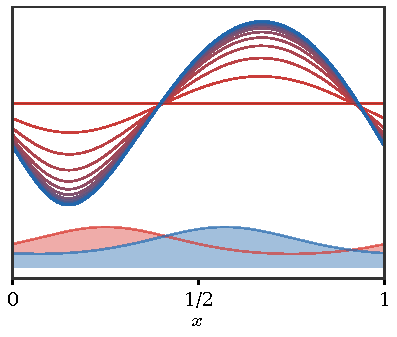
\includegraphics[width=.46\linewidth]{figures/sinkhorn-continuous-epsilon-flow/unimodal.pdf} &
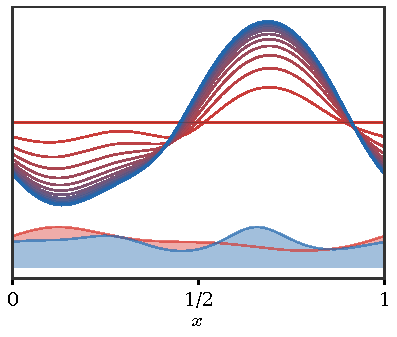
\includegraphics[width=.46\linewidth]{figures/sinkhorn-continuous-epsilon-flow/multimodal.pdf} \\[-.1em]
\small translated smooth bump & \small oscillatory split density
\end{tabular}
\caption{\emph{Continuous \(\varepsilon\)-Sinkhorn flow in one dimension.} The curves are snapshots of the gauge-fixed potential $u_t$, initialized at $u_0=0$, under the parabolic Monge--Ampere equation~\textup{(CES)} obtained from Berman's high-resolution, vanishing-temperature Sinkhorn scaling. Time is encoded from red to blue. The faint bottom silhouettes show the source density in red and the target density in blue. The examples are deliberately smooth so that the finite-difference evolution remains inside the monotone regime $1+u_t''>0$.}
\index{Monge-Ampere@Monge--Amp\`ere!parabolic equation}% strictindex
\index{Sinkhorn!continuous flow}% strictindex
\label{fig:sinkhorn-continuous-epsilon-flow}
\end{figure}

%%%%%%%%%%%%%%%%%%%%%%%%%%%%%%%%%%%%%%%%%%%%%%%%%%%%%%%%%%%%%%%%%%%%%%%%%%%
\section{Monotone Clearing Beyond Variational Sinkhorn}
\index{M-function}% strictindex
\index{non-variational scaling}% strictindex
\index{Sinkhorn!scaling}% strictindex
\label{sec-mfunction-scaling}

The preceding sections mostly used variational structure: Sinkhorn is alternating KL projection, coordinate ascent on a dual objective, or a contraction in a projective metric. There is another, more algebraic, convergence mechanism which keeps the scaling form but discards the existence of an objective. In Galichon's equilibrium-flow viewpoint, and in related work on substitutability and inverse isotonicity, one studies nonlinear market-clearing equations whose Jacobian has a substitute sign structure~\cite{GalichonJacquet2024Substitutability,GalichonSamuelsonVernet2022Monotone}. This is the nonlinear analogue of the classical theory of nonsingular M-matrices and M-functions~\cite{MoreRheinboldt1973PSFunctions,Plemmons1977MMatrix}. The relevance for OT is that Sinkhorn is the canonical scaling example, but the same monotone-clearing proof also covers fixed-point equations that are not first-order conditions of any convex regularized transport problem.
\index{market clearing}% strictindex
\index{substitutability}% strictindex
\index{gross substitutes}% strictindex

\paragraph{Two-block clearing maps.}
Write the unknowns as two blocks \(z=(u,v)\in\RR^n\times\RR^m\), where \(u\) and \(v\) will later be signed log-scalings. Let
\index{log-scaling}% strictindex
\[
	Q(z)=\big(Q^\alpha(u,v),Q^\beta(u,v)\big)
	\in\RR^n\times\RR^m
\]
be a continuous clearing map. The parallel coordinate-clearing map \(T\) is defined by solving, for each coordinate,
\[
	Q_\ell\big(T_\ell(z),z_{-\ell}\big)=0,
	\qquad 1\leq \ell\leq n+m.
\]
This is the Jacobi version: all coordinates are cleared against the old values of the other coordinates. In two-block scaling problems, all coordinates in \(u\) decouple when \(v\) is fixed, and all coordinates in \(v\) decouple when \(u\) is fixed. The more common alternating Sinkhorn sweep is the Gauss--Seidel composition of these two block clearings; the order argument below is stated for the parallel map to keep the notation short. The same construction extends to any finite number of blocks.

\begin{defn}[Z-functions and M-functions]\label{def-mfunctions}
\index{Z-function}% strictindex
\index{M-function}% strictindex
\index{diagonal isotonicity}% strictindex
\index{inverse isotonicity}% strictindex
	Let \(D\subset\RR^N\) be an order interval. A map \(Q:D\to\RR^N\) is diagonally isotone if \(Q_\ell(z_\ell,z_{-\ell})\) is nondecreasing in \(z_\ell\) for every \(\ell\). It is a Z-function if increasing the other coordinates cannot increase the \(\ell\)-th component:
	\[
		z_{-\ell}\leq z'_{-\ell}
		\quad\Longrightarrow\quad
		Q_\ell(z_\ell,z_{-\ell})\geq Q_\ell(z_\ell,z'_{-\ell}).
	\]
	For a \(C^1\) map this means \(\partial Q_\ell/\partial z_k\leq0\) for \(k\neq\ell\). An M-function is a Z-function which is inverse isotone:
	\[
		Q(z)\leq Q(z')
		\quad\Longrightarrow\quad
		z\leq z'.
	\]
	A vector \(z\) is a subsolution if \(Q(z)\leq0\), and a supersolution if \(Q(z)\geq0\).
\index{subsolution}% strictindex
\index{supersolution}% strictindex
\index{order interval}% strictindex
\end{defn}

The M-function assumption says that cross-effects have the sign of substitutes, and that own effects dominate them strongly enough to prevent a global reversal of order. Galichon, Samuelson and Vernet formulate this idea through nonreversingness and unified gross substitutes; for single-valued maps this is the inverse-isotone structure used below. A degenerate \(M_0\)-function keeps the same order structure but allows a null gauge direction, which is exactly what happens for balanced Sinkhorn before a potential normalization is imposed.
\index{M0-function}% strictindex
\index{gauge direction}% strictindex

\begin{thm}[Monotone convergence of coordinate clearing]\label{thm-mfunction-jacobi-convergence}
\index{coordinate clearing}% strictindex
\index{Jacobi iteration}% strictindex
\index{M-function}% strictindex
	Let \(D=[\underline z,\overline z]\subset\RR^N\) be a closed order interval, with \(\underline z\) a subsolution and \(\overline z\) a supersolution. Assume that \(Q:D\to\RR^N\) is continuous, diagonally isotone and an M-function. Assume also that, for every \(z\in D\) and every \(\ell\), the scalar clearing equation \(Q_\ell(\xi,z_{-\ell})=0\) has a unique solution \(\xi\in[\underline z_\ell,\overline z_\ell]\). Then \(Q(z)=0\) has a unique solution \(z^\star\in D\). The Jacobi coordinate-clearing iterates starting from any subsolution in \(D\) increase monotonically to \(z^\star\), while those starting from any supersolution in \(D\) decrease monotonically to \(z^\star\).
\end{thm}

\begin{proof}
	Let \(T\) be the coordinate-clearing map. If \(z\in D\) is a subsolution, then \(Q_\ell(z_\ell,z_{-\ell})\leq0=Q_\ell(T_\ell(z),z_{-\ell})\). Diagonal isotonicity and uniqueness of the scalar zero give \(z_\ell\leq T_\ell(z)\) for every \(\ell\), hence \(z\leq T(z)\). Since \(Q\) is a Z-function,
	\[
		Q_\ell(T(z))
		\leq
		Q_\ell(T_\ell(z),z_{-\ell})
		=0,
	\]
	so \(T(z)\) is again a subsolution. Since every subsolution lies below every supersolution by inverse isotonicity, \(T(z)\leq\overline z\), and therefore \(T(z)\in D\). The supersolution argument is the same with all inequalities reversed. The lower and upper iterates are thus monotone and trapped in the compact interval \(D\). Their limits exist, and passing to the limit in the identities \(Q_\ell(z_\ell^{(k+1)},z_{-\ell}^{(k)})=0\) gives \(Q(z^\star)=0\). If \(z\) and \(z'\) were two zeros in \(D\), then \(Q(z)\leq Q(z')\) and \(Q(z')\leq Q(z)\); inverse isotonicity gives \(z=z'\).
\end{proof}

\begin{prop}[Smooth M-matrix certificate]\label{prop-smooth-mfunction-certificate}
\index{M-matrix}% strictindex
\index{Z-matrix}% strictindex
\index{diagonal dominance}% strictindex
	Let \(D\subset\RR^N\) be a convex order interval and let \(Q:D\to\RR^N\) be \(C^1\). Assume that \(DQ(z)\) has nonpositive off-diagonal entries for every \(z\in D\). If there exists \(\lambda\gg0\) such that
	\[
		\lambda^\top DQ(z)\gg0
		\qquad\text{for all } z\in D,
	\]
	or equivalently
	\[
		\lambda_\ell\frac{\partial Q_\ell}{\partial z_\ell}(z)
		>
		\sum_{k\neq \ell}\lambda_k
		\left|\frac{\partial Q_k}{\partial z_\ell}(z)\right|,
		\qquad 1\leq \ell\leq N,
	\]
	then \(Q\) is an M-function on \(D\).
\end{prop}

\begin{proof}
	The off-diagonal sign gives the Z-property by integrating the partial derivatives along coordinatewise increasing segments. The displayed inequalities imply that each \(DQ(z)\) is a strictly weighted column diagonally dominant Z-matrix, hence a nonsingular M-matrix; in particular \(DQ(z)^{-1}\geq0\) for each fixed \(z\)~\cite{Plemmons1977MMatrix}. For two points \(z,z'\in D\), set
	\(A=\int_0^1 DQ\big(z'+t(z-z')\big)\,\d t\).
	The matrix \(A\) has the same Z-sign pattern and the same strict weighted diagonal dominance, so it is again a nonsingular M-matrix and \(A^{-1}\geq0\). Since \(Q(z)-Q(z')=A(z-z')\), the implication \(Q(z)\leq Q(z')\) gives \(z-z'=A^{-1}(Q(z)-Q(z'))\leq0\). This is inverse isotonicity. The positive diagonal entries also give diagonal isotonicity.
\end{proof}

\paragraph{Sinkhorn as the canonical \(M_0\)-system.}
\index{M0-function}% strictindex
\index{Sinkhorn!scaling}% strictindex
Let \(\K=\exp(-\C/\epsilon)>0\), and write the entropic plan as
\[
	\P_{i,j}=r_i\K_{i,j}s_j,
	\qquad r_i=e^{u_i},\qquad s_j=e^{-v_j}.
\]
The signed convention \(v=-\log s\) makes the clearing map
\[
	Q_i^\alpha(u,v)=\sum_j\K_{i,j}e^{u_i-v_j}-a_i,
	\qquad
	Q_j^\beta(u,v)=b_j-\sum_i\K_{i,j}e^{u_i-v_j}.
\]
The equations \(Q=0\) are the row and column constraints \(\P\ones=\a\) and \(\P^\top\ones=\b\), and the coordinate-clearing equations give the usual Sinkhorn scalings
\index{row constraint}% strictindex
\index{column constraint}% strictindex
\index{coordinate clearing}% strictindex
\[
	r_i^+=\frac{a_i}{\sum_j\K_{i,j}s_j},
	\qquad
	s_j^+=\frac{b_j}{\sum_i\K_{i,j}r_i}.
\]
The Jacobian has positive diagonal terms and nonpositive off-diagonal terms:
\[
	\frac{\partial Q_i^\alpha}{\partial u_i}=\sum_jP_{i,j},
	\qquad
	\frac{\partial Q_i^\alpha}{\partial v_j}=-\P_{i,j},
	\qquad
	\frac{\partial Q_j^\beta}{\partial v_j}=\sum_iP_{i,j},
	\qquad
	\frac{\partial Q_j^\beta}{\partial u_i}=-\P_{i,j}.
\]
Its column sums vanish, which reflects the gauge invariance \((u,v)\mapsto(u+c\ones,v+c\ones)\). Thus balanced Sinkhorn is naturally an \(M_0\)-system. Fixing one log-scaling coordinate removes this null direction and turns the reduced Jacobian into a principal minor of the weighted bipartite graph Laplacian. Under the connected-support condition, which is automatic here because \(\K>0\), this minor is a nonsingular M-matrix, so the M-function convergence mechanism applies on the gauge-fixed variables. This order-theoretic reading complements the variational and Hilbert-metric proofs above, and also appears in the link between Sinkhorn scaling and choice models~\cite{QuGalichonUgander2023SinkhornChoice}.
\index{Sinkhorn!scaling}% strictindex
\index{M-matrix}% strictindex
\index{gauge invariance}% strictindex

\begin{example}[Lossy Sinkhorn clearing with outside options]\label{ex-lossy-sinkhorn-clearing}
\index{lossy Sinkhorn clearing}% strictindex
\index{non-variational scaling}% strictindex
	The following OT-shaped clearing model is deliberately minimal. It keeps a positive transport kernel and multiplicative scalings, but introduces outside options and lossy arrivals. It should be read as a toy absorptive matching model rather than as a new transport distance. Let \(0<\eta_{i,j}\leq1\), \(\sigma_i>0\), \(\tau_j>0\), and set
\index{outside option}% strictindex
\index{absorptive matching}% strictindex
\index{loss factor}% strictindex
	\[
		\P_{i,j}=r_i\K_{i,j}s_j,\qquad r_i=e^{u_i},\qquad s_j=e^{-v_j}.
	\]
	The clearing equations are
	\[
		\sigma_i r_i+\sum_jP_{i,j}=a_i,
		\qquad
		\tau_j s_j+\sum_i\eta_{i,j}\P_{i,j}=b_j.
	\]
	They say that source mass can exit through an outside sink, while target demand can be met either by effective arrivals or by a local outside source. The coordinate-clearing update is still Sinkhorn-like:
	\[
		r_i^+=\frac{a_i}{\sigma_i+\sum_j\K_{i,j}s_j},
		\qquad
		s_j^+=\frac{b_j}{\tau_j+\sum_i\eta_{i,j}\K_{i,j}r_i}.
	\]
	In the variables \((u,v)\), the off-diagonal derivatives again have the Z-sign. On the invariant domain \(r_i\leq a_i/\sigma_i\), the simple sufficient condition
	\[
		\tau_j>\sum_i(1-\eta_{i,j})\K_{i,j}\frac{a_i}{\sigma_i},
		\qquad 1\leq j\leq m,
	\]
	implies the weighted diagonal-dominance certificate \(\ones^\top DQ\gg0\), hence Proposition~\ref{prop-smooth-mfunction-certificate} shows that the system is an M-function on that domain. Indeed, for the clearing map \(Q_i^\alpha=\sigma_i r_i+\sum_jP_{i,j}-a_i\) and \(Q_j^\beta=b_j-\tau_j s_j-\sum_i\eta_{i,j}\P_{i,j}\), the column sums of the Jacobian are
	\[
		\sigma_i r_i+\sum_j(1-\eta_{i,j})\P_{i,j}>0,
		\qquad
		\tau_j s_j-\sum_i(1-\eta_{i,j})\P_{i,j}
		=
		s_j\left(\tau_j-\sum_i(1-\eta_{i,j})\K_{i,j}r_i\right)>0.
	\]
	The model is generally non-variational. If \(Q=\nabla\mathcal E\) for a \(C^2\) potential, the cross-partials would satisfy
	\[
		\frac{\partial Q_i^\alpha}{\partial v_j}
		=
		\frac{\partial Q_j^\beta}{\partial u_i}.
	\]
	Here this would force \(-\P_{i,j}=-\eta_{i,j}\P_{i,j}\) on every active arc, hence \(\eta_{i,j}=1\). Lossy arrivals therefore destroy exactness of the one-form \(\sum_\ell Q_\ell\,\d z_\ell\), while preserving the monotone clearing structure.
\index{one-form}% strictindex
\end{example}

Figure~\ref{fig:sinkhorn-mfunctions-nonvariational-scaling} shows this mechanism on two empirical Gaussian mixtures in \(\RR^2\). In the figure, the outside coefficients are written as \(\sigma_i=\rho\bar\sigma_i\) and \(\tau_j=\rho\bar\tau_j\), and the columns increase the common scale \(\rho\). The visual point is not an optimization benchmark but the persistence of a well-behaved Sinkhorn-shaped fixed point outside the variational OT setting.

\begin{figure}[ht]
\centering
\setlength{\tabcolsep}{4pt}
\begin{tabular}{@{}c@{}}
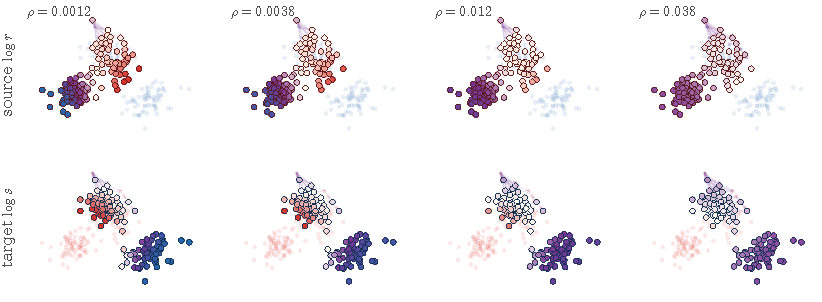
\includegraphics[width=.88\linewidth]{figures/sinkhorn-mfunctions-nonvariational-scaling/uniform-outside.pdf} \\[-.15em]
\small uniform outside coefficients \\[.25em]
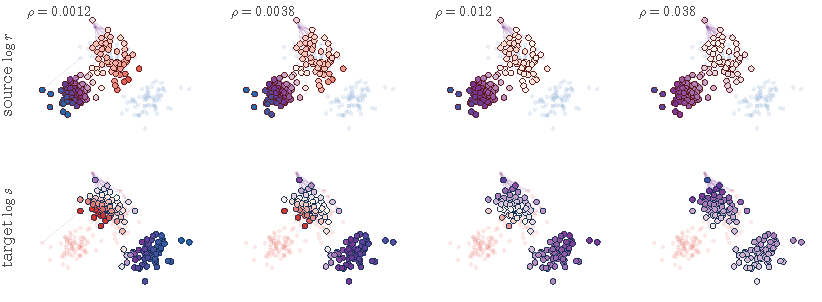
\includegraphics[width=.88\linewidth]{figures/sinkhorn-mfunctions-nonvariational-scaling/spatial-outside.pdf} \\[-.15em]
\small spatially varying outside coefficients
\end{tabular}
\caption{\emph{Non-variational lossy Sinkhorn scaling on two Gaussian-mixture point clouds.} Across columns, the outside-option scale \(\rho\) increases in \(\sigma\) and \(\tau\). Colors show centered log-scalings, \(\log r-\langle\log r\rangle\) on the source row and \(\log s-\langle\log s\rangle\) on the target row; faint violet links mark the largest entries of the induced effective plan. The upper panel uses uniform outside coefficients, while the lower panel uses spatially varying outside coefficients and directional loss factors. The updates are Sinkhorn-like row and column clearings, but the loss factors \(\eta_{i,j}\neq1\) break the cross-partial symmetry required by a convex potential.}
\index{lossy Sinkhorn clearing}% strictindex
\index{M-function}% strictindex
\label{fig:sinkhorn-mfunctions-nonvariational-scaling}
\end{figure}

%%%


%%%%%%%%%%%%%%%%%%%%%%%%%%%%%%%%%%%%%%%%%%%%%%%%%%%%%%%%%%%%%%%%%%%%%%%%%%%
